% Options for packages loaded elsewhere
\PassOptionsToPackage{unicode}{hyperref}
\PassOptionsToPackage{hyphens}{url}
\PassOptionsToPackage{dvipsnames,svgnames,x11names}{xcolor}
%
\documentclass[
]{article}

\usepackage{amsmath,amssymb}
\usepackage{iftex}
\ifPDFTeX
  \usepackage[T1]{fontenc}
  \usepackage[utf8]{inputenc}
  \usepackage{textcomp} % provide euro and other symbols
\else % if luatex or xetex
  \usepackage{unicode-math}
  \defaultfontfeatures{Scale=MatchLowercase}
  \defaultfontfeatures[\rmfamily]{Ligatures=TeX,Scale=1}
\fi
\usepackage{lmodern}
\ifPDFTeX\else  
    % xetex/luatex font selection
\fi
% Use upquote if available, for straight quotes in verbatim environments
\IfFileExists{upquote.sty}{\usepackage{upquote}}{}
\IfFileExists{microtype.sty}{% use microtype if available
  \usepackage[]{microtype}
  \UseMicrotypeSet[protrusion]{basicmath} % disable protrusion for tt fonts
}{}
\makeatletter
\@ifundefined{KOMAClassName}{% if non-KOMA class
  \IfFileExists{parskip.sty}{%
    \usepackage{parskip}
  }{% else
    \setlength{\parindent}{0pt}
    \setlength{\parskip}{6pt plus 2pt minus 1pt}}
}{% if KOMA class
  \KOMAoptions{parskip=half}}
\makeatother
\usepackage{xcolor}
\setlength{\emergencystretch}{3em} % prevent overfull lines
\setcounter{secnumdepth}{5}
% Make \paragraph and \subparagraph free-standing
\ifx\paragraph\undefined\else
  \let\oldparagraph\paragraph
  \renewcommand{\paragraph}[1]{\oldparagraph{#1}\mbox{}}
\fi
\ifx\subparagraph\undefined\else
  \let\oldsubparagraph\subparagraph
  \renewcommand{\subparagraph}[1]{\oldsubparagraph{#1}\mbox{}}
\fi


\providecommand{\tightlist}{%
  \setlength{\itemsep}{0pt}\setlength{\parskip}{0pt}}\usepackage{longtable,booktabs,array}
\usepackage{calc} % for calculating minipage widths
% Correct order of tables after \paragraph or \subparagraph
\usepackage{etoolbox}
\makeatletter
\patchcmd\longtable{\par}{\if@noskipsec\mbox{}\fi\par}{}{}
\makeatother
% Allow footnotes in longtable head/foot
\IfFileExists{footnotehyper.sty}{\usepackage{footnotehyper}}{\usepackage{footnote}}
\makesavenoteenv{longtable}
\usepackage{graphicx}
\makeatletter
\def\maxwidth{\ifdim\Gin@nat@width>\linewidth\linewidth\else\Gin@nat@width\fi}
\def\maxheight{\ifdim\Gin@nat@height>\textheight\textheight\else\Gin@nat@height\fi}
\makeatother
% Scale images if necessary, so that they will not overflow the page
% margins by default, and it is still possible to overwrite the defaults
% using explicit options in \includegraphics[width, height, ...]{}
\setkeys{Gin}{width=\maxwidth,height=\maxheight,keepaspectratio}
% Set default figure placement to htbp
\makeatletter
\def\fps@figure{htbp}
\makeatother
% definitions for citeproc citations
\NewDocumentCommand\citeproctext{}{}
\NewDocumentCommand\citeproc{mm}{%
  \begingroup\def\citeproctext{#2}\cite{#1}\endgroup}
\makeatletter
 % allow citations to break across lines
 \let\@cite@ofmt\@firstofone
 % avoid brackets around text for \cite:
 \def\@biblabel#1{}
 \def\@cite#1#2{{#1\if@tempswa , #2\fi}}
\makeatother
\newlength{\cslhangindent}
\setlength{\cslhangindent}{1.5em}
\newlength{\csllabelwidth}
\setlength{\csllabelwidth}{3em}
\newenvironment{CSLReferences}[2] % #1 hanging-indent, #2 entry-spacing
 {\begin{list}{}{%
  \setlength{\itemindent}{0pt}
  \setlength{\leftmargin}{0pt}
  \setlength{\parsep}{0pt}
  % turn on hanging indent if param 1 is 1
  \ifodd #1
   \setlength{\leftmargin}{\cslhangindent}
   \setlength{\itemindent}{-1\cslhangindent}
  \fi
  % set entry spacing
  \setlength{\itemsep}{#2\baselineskip}}}
 {\end{list}}
\usepackage{calc}
\newcommand{\CSLBlock}[1]{\hfill\break\parbox[t]{\linewidth}{\strut\ignorespaces#1\strut}}
\newcommand{\CSLLeftMargin}[1]{\parbox[t]{\csllabelwidth}{\strut#1\strut}}
\newcommand{\CSLRightInline}[1]{\parbox[t]{\linewidth - \csllabelwidth}{\strut#1\strut}}
\newcommand{\CSLIndent}[1]{\hspace{\cslhangindent}#1}

\makeatletter
\@ifpackageloaded{caption}{}{\usepackage{caption}}
\AtBeginDocument{%
\ifdefined\contentsname
  \renewcommand*\contentsname{Table of contents}
\else
  \newcommand\contentsname{Table of contents}
\fi
\ifdefined\listfigurename
  \renewcommand*\listfigurename{List of Figures}
\else
  \newcommand\listfigurename{List of Figures}
\fi
\ifdefined\listtablename
  \renewcommand*\listtablename{List of Tables}
\else
  \newcommand\listtablename{List of Tables}
\fi
\ifdefined\figurename
  \renewcommand*\figurename{Figure}
\else
  \newcommand\figurename{Figure}
\fi
\ifdefined\tablename
  \renewcommand*\tablename{Table}
\else
  \newcommand\tablename{Table}
\fi
}
\@ifpackageloaded{float}{}{\usepackage{float}}
\floatstyle{ruled}
\@ifundefined{c@chapter}{\newfloat{codelisting}{h}{lop}}{\newfloat{codelisting}{h}{lop}[chapter]}
\floatname{codelisting}{Listing}
\newcommand*\listoflistings{\listof{codelisting}{List of Listings}}
\makeatother
\makeatletter
\makeatother
\makeatletter
\@ifpackageloaded{caption}{}{\usepackage{caption}}
\@ifpackageloaded{subcaption}{}{\usepackage{subcaption}}
\makeatother
\ifLuaTeX
  \usepackage{selnolig}  % disable illegal ligatures
\fi
\usepackage{bookmark}

\IfFileExists{xurl.sty}{\usepackage{xurl}}{} % add URL line breaks if available
\urlstyle{same} % disable monospaced font for URLs
\hypersetup{
  pdftitle={T is for Topology},
  pdfauthor={Tanya Strydom; Jennifer A. Dunne; Timothée Poisot; Andrew P. Beckerman},
  pdfkeywords={food web, network construction},
  colorlinks=true,
  linkcolor={blue},
  filecolor={Maroon},
  citecolor={Blue},
  urlcolor={Blue},
  pdfcreator={LaTeX via pandoc}}


\title{T is for Topology}
\author{Tanya Strydom %
%
\textsuperscript{%
%
1%
}%
; Jennifer A. Dunne %
%
\textsuperscript{%
%
2%
}%
; Timothée Poisot %
%
\textsuperscript{%
3,%
4%
}%
; Andrew P. Beckerman %
%
\textsuperscript{%
%
1%
}%
}
\date{2024-05-02}

\usepackage{setspace}
\usepackage[left,pagewise]{lineno}
\usepackage[letterpaper]{geometry}

\usepackage[nolists,noheads,markers]{endfloat}
\geometry{margin=2.5cm}

\begin{document}

\thispagestyle{empty}
{\bfseries\sffamily\Large T is for Topology}
\vfil
Tanya Strydom %
%
\textsuperscript{%
%
1%
}%
; Jennifer A. Dunne %
%
\textsuperscript{%
%
2%
}%
; Timothée Poisot %
%
\textsuperscript{%
3,%
4%
}%
; Andrew P. Beckerman %
%
\textsuperscript{%
%
1%
}%

\vfil
{\small
\textbf{Abstract:} Although it has been acknowledged that communities
consist not only of co-occurring species but that they also interact
being able to quantify those interactions and assemble them into
interaction networks has been a limiting factor in the integration of
network ecology into other fields of ecology. As the field of network
ecology has matured there has been an accompanying expansion in the
development of theory and tools that are centred around generating
networks or predicting the interactions between species. Notably many of
these tools have been developed with different underlying philosophies,
ideas, and mechanisms as to what structures the interactions between
species. It is thus critically important that those wanting to adopt
these network generating tools be aware of how the the specific
questions being asked maps to the underlying assumptions made when
generating networks, as well as the limitations of how the
networks/interactions are delimited. Here we provide an overview of the
canonical network generating models, comparing and contrasting the
underlying assumptions, data requirements, and resulting network
predictions made by the different families in an attempt to provide
guidance for those interested in adopting the generation of networks
into their workflow. {[}R1. a discussion on the underlying assumptions
we are making when we delimit a network{]}. {[}R2. an overview of how
the different model families differ - ordination space/benchmarking{]}.
{[}R3. identifying the relevant questions/bodies of theory that the
networks generated by different families are suited to answer{]}. When
choosing to construct an interaction network the researcher is faced
with many assumptions and considerations that should be made and it is
important to be aware of these limitations to avoid constructing
(something poetic to capture the idea of falsity/false idols). Being
aware of these choices is particularly important as the availability of
these tools grows and network ecology starts to be adopted into other
aspects of ecology and conservation biology.
\vfil
\textbf{Keywords:} %
food web, %
network construction%
}
\clearpage
\setcounter{page}{1}
\doublespacing
\linenumbers

It can be argued that the interaction between species (or individuals)
is one of the main determinants of the emergent properties that are
studied in other fields of ecology, \emph{e.g.,} the range of plant will
be determined by the range of its pollinator, and although the
importance of species interactions and the resulting networks that they
form has been an acknowledged part of the ecological canon since the
penning of the `entangled bank' (Darwin, 1859) (if not even earlier,
stemming from Greek Antiquity (Thanos, 1994)), the adoption of network
ecology into other disciplines of ecology has been limited. This has
primarily been driven by two limitations; firstly, it is extremely
challenging to actually record species interactions in the field
(Jordano, 2016a, 2016b), which has resulted in a limited coverage of
`real world' interaction data (Poisot et al., 2021), and secondly has
been the need to develop terminology and tools that help us to
construct, conceptualise, and analyse these networks. Although recording
interactions in the field remains a challenge, the development of both
practical tools (\emph{i.e.,} tools that help us to record or measure
interactions, Pringle \& Hutchinson, 2020), as well as discussions
around the development of tools to predict or infer them
(Morales-Castilla et al., 2015; Strydom, Catchen, et al., 2021), has
allowed us to begin filling in these `global gaps', albeit in a,
potentially, more synthetic manner (Poisot, Gravel, et al., 2016).
Additionally, there has been extensive development in in the ways in
which we formalise networks (Dale \& Fortin, 2010; Fortin et al., 2012),
and the tools and language that we use to quantify the structure and
properties of networks (Delmas et al., 2019). All together these tools
mean that, as a field, network ecology can (and should) be integrated
into the broader fields of ecology (\emph{e.g.,} Thuiller et al., 2024)
and conservation biology (\emph{e.g.,} Bhatia et al., 2023). However (as
with any new tool or model), it is important that one has a firm grasp
of how the underlying philosophy that underpins the construction of
networks (particularly synthetic ones) can have an impact on the
interpretation of the questions being asked. In this manuscript we will
discuss three themes that should help provide clarity and understanding
for those wishing to take a step into network (particularly food web)
ecology this includes; thinking about and understanding the underlying
assumptions that are made when we attempt to delimit and describe a food
webs, a synthesis of the different families of tools that are commonly
used to construct food webs, and a discussion linking network ecology to
some of the outstanding questions in ecology.

\begin{figure}

\centering{

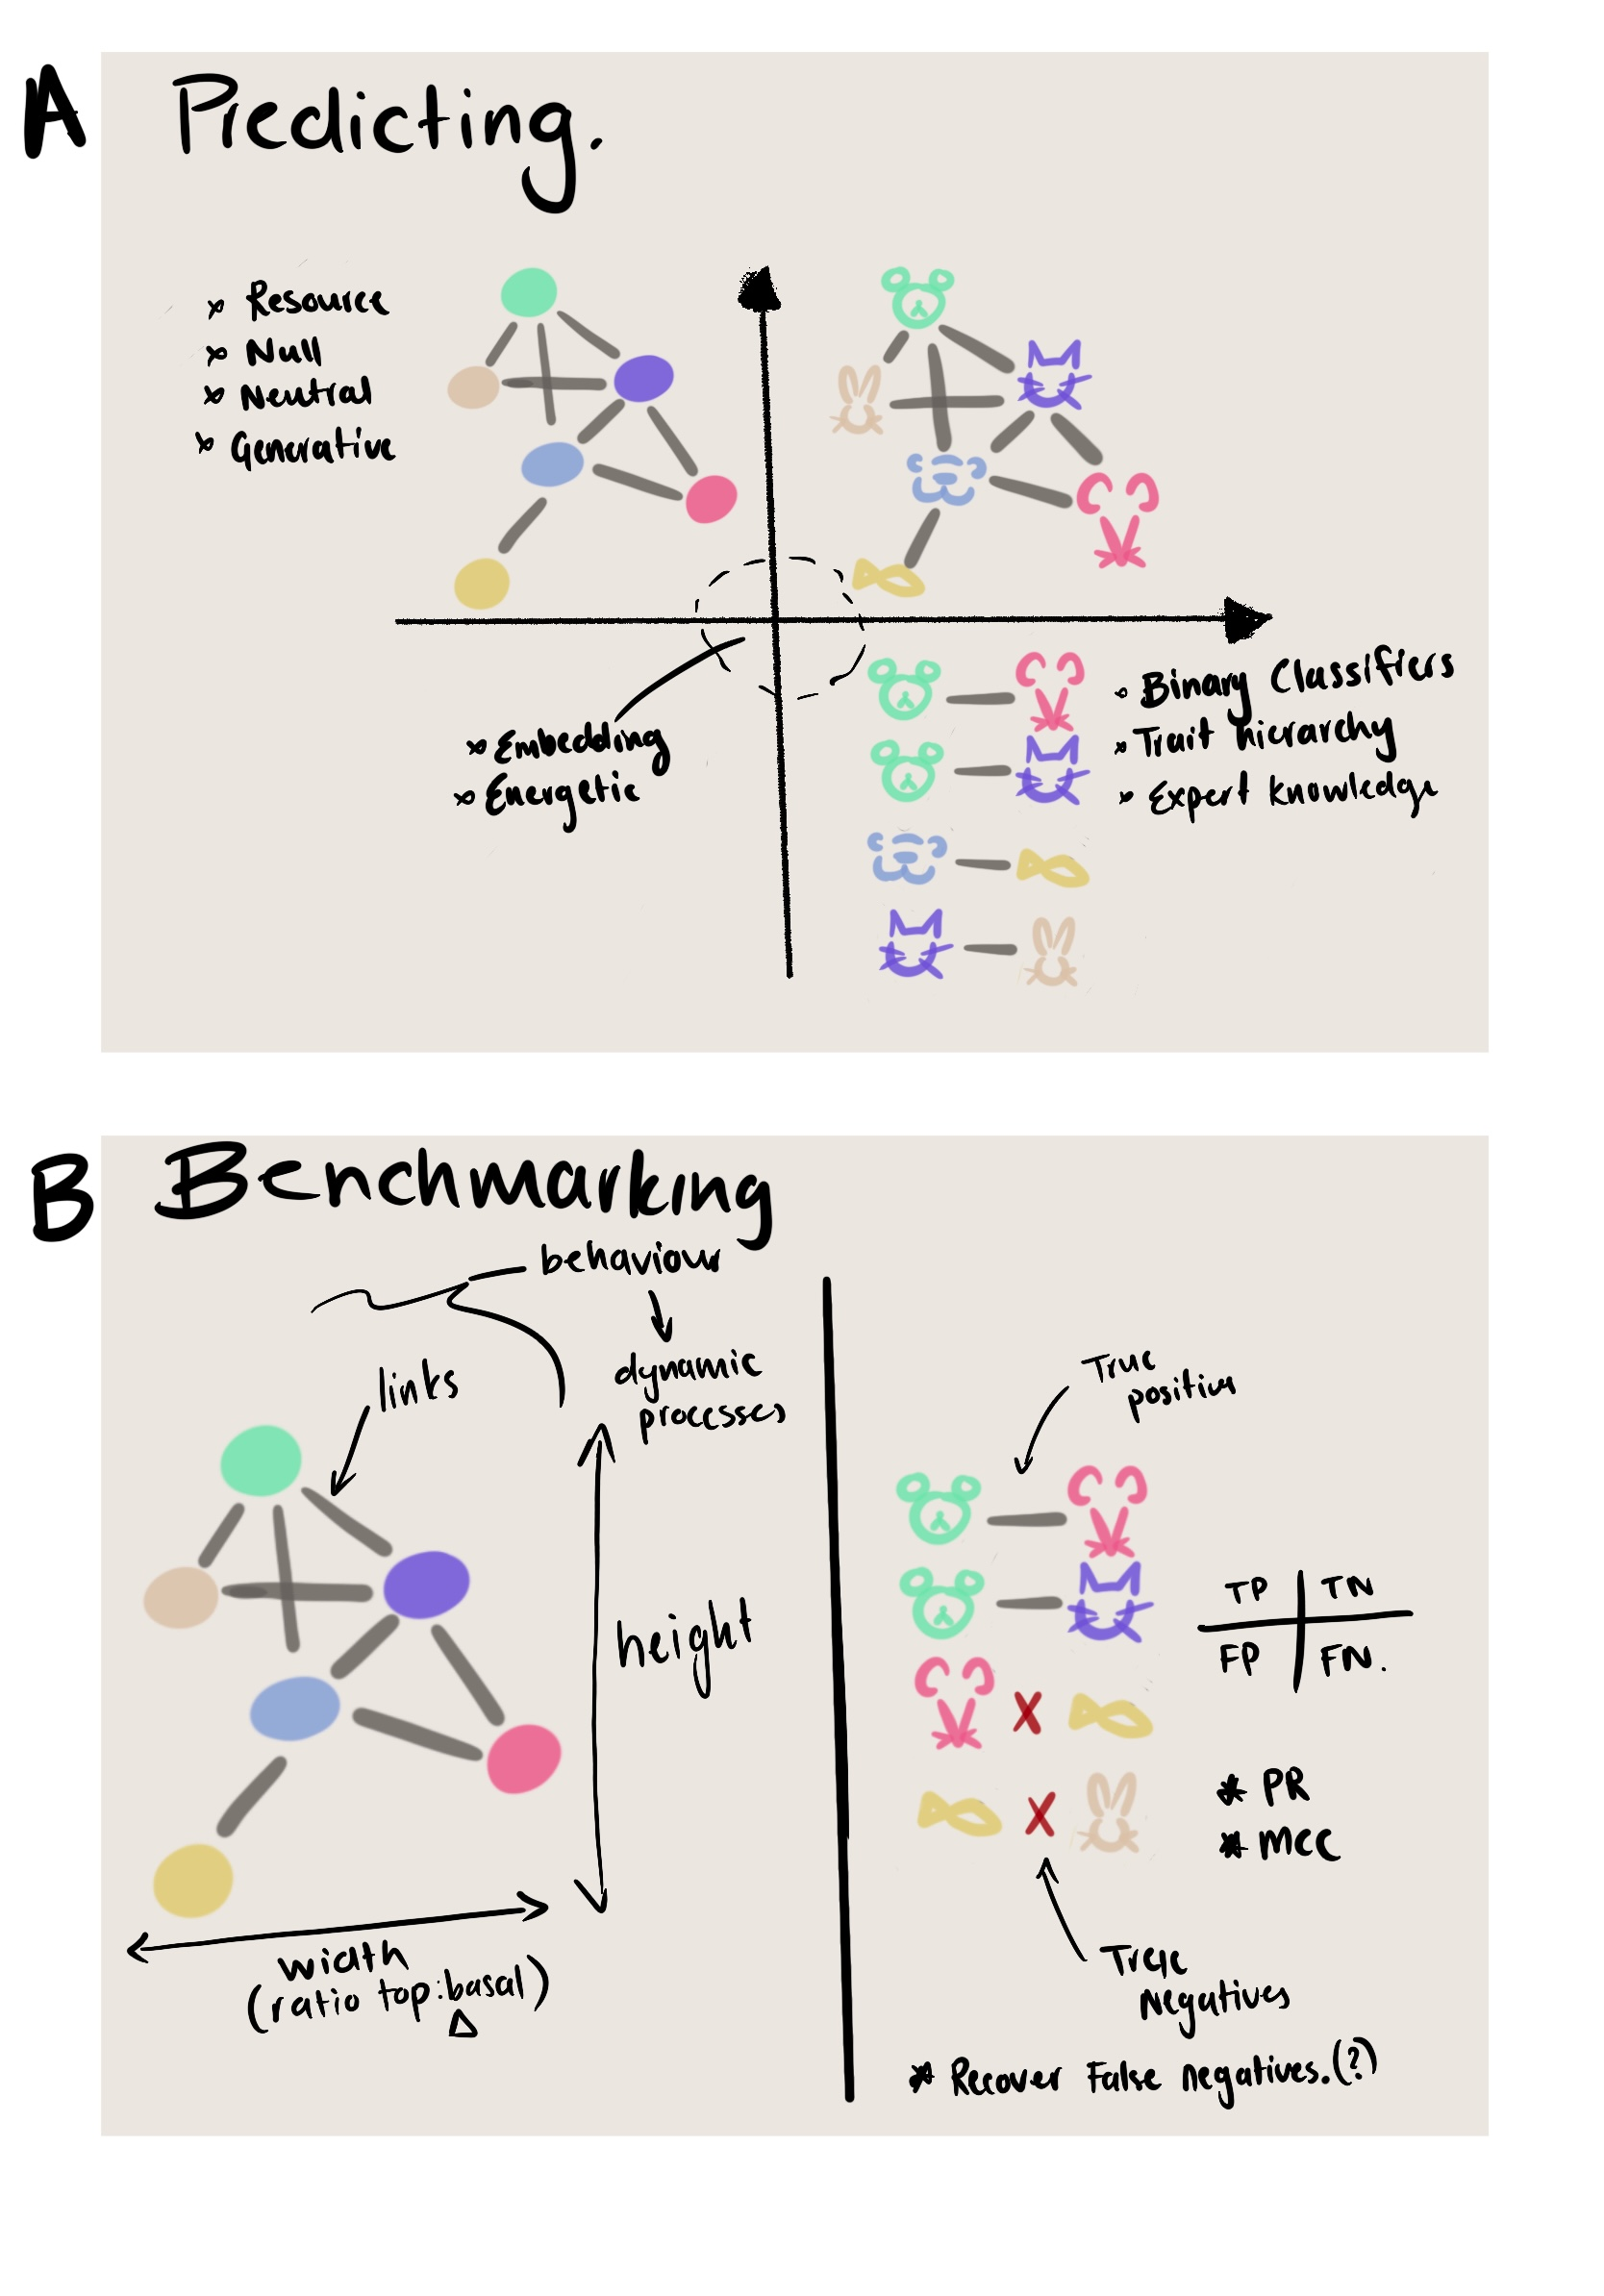
\includegraphics{images/concept.jpeg}

}

\caption{\label{fig-concept}Conceptual figure of the `network
prediction'. Panel A shows where the model families fall in the the
context of being models that predict networks or models that predict
interactions space. Panel B serves to highlight the characteristics one
might like to `test'/benchmark for a model based on it being either a
network or interaction predicting model}

\end{figure}%

\section{The anatomy of a food web}\label{sec-network-anatomy}

Although we specifically focus on food webs (interactions representing
feeding links) it is beneficial to take a step back and acknowledge the
diversity of form that an interaction network can encapsulate. The idea
of an interaction network seems simple, it is the representation of the
interactions (edges) between species (nodes), the definition of an
`edge' and a `node', as well as the scale at which they are aggregated
can take many forms. As highlighted in Poisot, Stouffer, et al. (2016)
networks can be constructed at the population (the links between
individuals), community (the links between species), or metacommunity
(fluxes between locations) level. Even if we are to limit our definition
of a network to represent community-level processes there are still many
ways to define what is captured by the edges and nodes {[}insert some
e.g.{]}. It is thus clear that the way that a network is coded
(constructed) can influence the resulting observations and conclusions
that are made (Brimacombe et al., 2023; Proulx et al., 2005), and it is
important to have a strong grasp of what information a network is
attempting to convey.

Even if one were to limit their scope to thinking of interaction
networks only in terms of food webs there are still many ways to define
the various components of the network, one needs to understand the
different intentions/assumptions that are made when a food web is
constructed. Although the main intention of a food web is to capture and
represent the feeding links between species there are many ways to
define the nodes (\emph{e.g.,} species or taxonomic group), edges
(\emph{e.g.} potential or realised feeding links), the magnitude of the
edges (\emph{e.g.,} binary vs probabilistic) and even how the network
itself is delimited (does it represent an aggregation of interactions
over time?, what is the spatial extent?). All these decisions will have
an impact on the resultant structure and potential use-cases of the
network.

\subsection{How do we define a node?}\label{how-do-we-define-a-node}

Although this may seem an elementary question in the context of food
webs --- a node should represent a species, the reality is that nodes
can often represent an aggregate of different (taxonomic) species - so
called `trophic species', and it is not uncommon that networks can have
nodes that represent both taxonomic and trophic species (\emph{e.g.,}
there are many that do the basal `plant/phytoplankton' node but include
at least one REF). Practical implications of how we are aggregating the
nodes is that the resolution may not always be `pixel perfect'
\emph{i.e.,} we may be unable to assess the co-extinction risk of a
species pair {[}mutualism ref, at least there should be one of them{]},
however there is value in having nodes that represent an aggregation of
species, as these convey a much more general overview of how the links
are distributed within the community.

\subsection{What is meant by an edge?}\label{what-is-meant-by-an-edge}

As discussed earlier there are many ways to define the links between
species --- even feeding links. At its core links within food webs can
be thought of as a representation of either the flow of a resource
{[}ref{]}, realised (Pringle, 2020) feeding links, potential (Dunne,
2006) feeding links, or energy flows{[}??{]} (Petchey et al., 2008). How
we quantify links will influence the resulting structure of the network
- and the inferences we will make thereof. For example taking a food web
that consists of links representing \emph{potential} feeding links
between species (\emph{i.e.,} a `present' interaction is one implies
that species \emph{a} has the ability to consume species \emph{b} but it
does not mean that this interaction is realised in the field) will be
meaningless if you are interested in understanding the flow of energy
through the system as the links within the network are over connected.
In addition to the various ways of defining the links between species
pairs there are also a myriad of ways in which the links themselves can
be quantified. Links between species are often treated as being present
or absent (\emph{i.e.,} binary) but it is also possible to use
probabilities (which quantifies how likely an interaction is to occur,
Poisot, Cirtwill, et al., 2016) or continuous measurements (which
quantifies the effect of one species on another, Berlow et al., 2004).
Although there is a clear argument for moving away from a purely binary
way of representing interactions {[}probabilities preprint{]} this of
course also means that there is an additional layer to the
interpretation these links.

\subsection{Aggregating networks}\label{aggregating-networks}

Here I think we need to talk about realised vs potential links (i.e.~the
concept of a metaweb) but also the idea that we are often aggregating
over time and space which makes boundaries and whatnot all a bit fuzzy

\begin{quote}
Cohen et al. (1985) states that \emph{``{[}Their{]} approach is more
like gross anatomy than like physiology\ldots{} that is, the gross
anatomy is frozen, rather than in motion.''}.
\end{quote}

\subsection{Putting the parts together; what does it
mean?}\label{putting-the-parts-together-what-does-it-mean}

It it clear that there are many ways to define, code, and construct food
webs, however what may be less clear is understanding \emph{why} there
is such a diversity of thought. Here it may be meaningful to
contextualise the different `types' of food webs within the larger
questions (or needs) that have been driving them. Some of the earliest
work on food webs was linked to the idea of niche space, and more
specifically, the idea of trophic niches and how this would influence
the dimensionality of a networks (Cohen, 1977). This introduced the idea
that a single dimension (the ``niche axis,'' Allesina et al., 2008)
constrains the interactions between species; in this instance it makes
sense to think of species in terms of what they consume and what they
are consumed by, as they are occupying the same space in the niche axis.
Networks that are defined in this way may be useful for understanding
how the flow of energy (resources) are constrained between `species',
particularly how it moves through the trophic levels. This `niche-based'
way of thinking might be beneficial when thinking about networks at the
structural level, and when trying to map large-scale processes
{[}ref?{]} however there was also a need to develop ways of thinking
that were more geared to thinking about why does species \emph{a}
predate species \emph{b}, broadly this is the result of two things; a
predator needs to have the correct traits to be able to capture, kill,
and consume, its prey (a mismatch between predator and prey is termed a
forbidden link, Jordano (2016b)) and it needs to be energetically
feasible {[}feeding ecology ref{]}. When we think of interactions in
these terms it makes sense that nodes are defined at the species level
(or at least as species that have the same traits and/or energy
content), however the links between them can be quantified in different
ways\ldots{} {[}this is lazy writing{]}

\emph{something, something, introducing that the same problem (different
philosophies) is also a thing that you need to think about when
aggregating interactions/generating networks.}

\section{Constructing ecological
networks}\label{constructing-ecological-networks}

\begin{quote}
maybe a more direct link here to the fact that when working with
networks its often synthetic ones \emph{i.e.,} the product of some sort
of modelling exercise; alternatively there has also been a push to
develop predictive tools to create hypothetical (but plausible) networks
for real world situations. Also talk about even deciding to create a
network from field observations is in and of itself still a `model' that
has assumptions\ldots{} for example decisions are made about delimiting,
aggregation, and observation, the idea of aggregating over time or
aggregating over space. Same can e said for different food web
generating tools , they have their own underlying rules and assumptions
that are made when constructing a food web, which will determine and
influence the resulting structure or inferred interactions (Petchey et
al., 2008)
\end{quote}

Arguably the need for methods and tools that can be used to construct
synthetic food webs arises from two different (but still aligned) places
of interest within the field of network ecology. On the one side sits
the researcher who is interested in generating a set of ecologically
plausible networks for the purpose of understanding some higher-level
process/concept (\emph{e.g.,} understanding energy flows) in a more
synthetic setting, whereby these networks do not require any level of
species specificity \emph{per se} and it is more the arrangement of the
nodes and links within the context of network structure that is of
value. This researcher is contrasted by one that is interested in
constructing real-world, location specific, interaction data for a
specific collection of species (community). This is driven by the need
for researchers to find alternative ways to infer the interactions
between species as a way to overcome the inherit challenges of
inventorying interactions in the field (see Morales-Castilla et al.
(2015) for a more mechanistic, and Strydom, Catchen, et al. (2021) for a
more statistical overview of ways to approach this specific issue). Of
course these two categories are not distinct, mutually exclusive, groups
but can rather be viewed as operating on a continuum ranging from a need
for generality (\emph{i.e.,} creating a network that, when taken in
aggregate, the distribution of links (interactions) between nodes
(species) are ecologically plausible) to a need for specificity
(\emph{i.e.,} local-level predictions between specific species pairs).
It is thus clear that (realistically) there will probably never be a
`best fit' tool that is able to construct a food web that will span the
entire range of needs, and rather the responsibility lies with the
researcher to be aware of not only the underlying philosophy of the
specific toolset (as this could have knock-on effects when using those
networks for downstream analyses/simulations; pers. comms. Beckerman,
2024), but also how well the tool is able to retrieve the specific
network or interaction properties that they desire.

\subsection{Model families}\label{model-families}

As there are many food web generating tools to choose from it is perhaps
useful to think about these tools in terms of families, where families
represent tools that have a similar methodology and (more importantly)
have the same underlying philosophies and assumptions that determine the
links betweens nodes as well as how these may be encoded, a summary of
these model families are presented in Table~\ref{tbl-families} and
discussed in more detail below. Although there have been efforts to
compare and contrast different models (\emph{e.g.,} Williams \&
Martinez, 2008 looked at `structural models'; and Pichler et al., 2020
looked at machine learning algorithms) there still lacks an overall
synthesis as to how the different model families differ from each other
- both in terms of what they are actually predicting as well as how well
they are preforming in the different facets of constructing a food web.

\begin{longtable}[]{@{}
  >{\raggedright\arraybackslash}p{(\columnwidth - 12\tabcolsep) * \real{0.1429}}
  >{\raggedright\arraybackslash}p{(\columnwidth - 12\tabcolsep) * \real{0.1429}}
  >{\raggedright\arraybackslash}p{(\columnwidth - 12\tabcolsep) * \real{0.1429}}
  >{\raggedright\arraybackslash}p{(\columnwidth - 12\tabcolsep) * \real{0.1429}}
  >{\raggedright\arraybackslash}p{(\columnwidth - 12\tabcolsep) * \real{0.1429}}
  >{\raggedright\arraybackslash}p{(\columnwidth - 12\tabcolsep) * \real{0.1429}}
  >{\raggedright\arraybackslash}p{(\columnwidth - 12\tabcolsep) * \real{0.1429}}@{}}
\caption{A summary of the different families of tools that can be used
to generate food webs, this includes a brief description of the
underlying philosophy of the family as well as how the different
elements (nodes and edges) of the generated network
represents.}\label{tbl-families}\tabularnewline
\toprule\noalign{}
\begin{minipage}[b]{\linewidth}\raggedright
Model family
\end{minipage} & \begin{minipage}[b]{\linewidth}\raggedright
Theory
\end{minipage} & \begin{minipage}[b]{\linewidth}\raggedright
Network predicted
\end{minipage} & \begin{minipage}[b]{\linewidth}\raggedright
Nodes represent
\end{minipage} & \begin{minipage}[b]{\linewidth}\raggedright
Links represent
\end{minipage} & \begin{minipage}[b]{\linewidth}\raggedright
Interaction
\end{minipage} & \begin{minipage}[b]{\linewidth}\raggedright
Key reference
\end{minipage} \\
\midrule\noalign{}
\endfirsthead
\toprule\noalign{}
\begin{minipage}[b]{\linewidth}\raggedright
Model family
\end{minipage} & \begin{minipage}[b]{\linewidth}\raggedright
Theory
\end{minipage} & \begin{minipage}[b]{\linewidth}\raggedright
Network predicted
\end{minipage} & \begin{minipage}[b]{\linewidth}\raggedright
Nodes represent
\end{minipage} & \begin{minipage}[b]{\linewidth}\raggedright
Links represent
\end{minipage} & \begin{minipage}[b]{\linewidth}\raggedright
Interaction
\end{minipage} & \begin{minipage}[b]{\linewidth}\raggedright
Key reference
\end{minipage} \\
\midrule\noalign{}
\endhead
\bottomrule\noalign{}
\endlastfoot
null & Network structure is random & structure & agnostic & feeding
links & binary & \\
neutral & Network structure is random, but species abundance plays a
role & structure & species & feeding links & binary & \\
resource & Networks are interval, species can be ordered on a `niche
axis' & structure & trophic species & subdivision of resource & binary &
Williams \& Martinez (2008) \\
generative & Networks are determined by their structural features &
structure & agnostic & links & binary & \\
energetic & Interactions are determined by foraging theory (feeding
links) & interactions & species & feeding links & quantitative & \\
graph embedding & Interactions can be predicted from the latent traits
of networks & interactions & species & potential feeding links &
probabilistic & Strydom et al. (2023) \\
trait matching & Interactions can be inferred by a mechanistic
framework/relationships & interactions & species & feeding links &
binary & Morales-Castilla et al. (2015) \\
binary classifiers & Interactions can be predicted by learning the
relationship between interactions and ecologically relevant predictors &
interactions & species & feeding links & binary & Pichler et al.
(2020) \\
expert knowledge & `Boots on the ground' ecological knowledge and
observations & interactions & species & feeding links & binary & \\
data scavenging & Webscraping to create networks from online databases &
interactions & species & feeding links & binary & \\
co-occurrence & co-occurrence patterns arise from interactions so we can
use these patterns to reverse engineer the interactions & co-occurrence
patterns & species & association links & binary & \\
\end{longtable}

\textbf{Null models:} The interactions between species occurs regardless
of the identity of the species (\emph{i.e.,} species have no agency) and
links are randomly distributed throughout the network. This family of
models is often used as a way of benchmarking things\ldots{} Broadly
there are two different approaches; Type I (Fortuna \& Bascompte, 2006),
where interactions happen proportionally to connectance and Type II
(Bascompte et al., 2003), where interactions happen proportionally to
the joint degree of the two species involved.

\textbf{Neutral models:} Can be tied to Hubble's (spellings but also
name??) neutral theory {[}ref, probably mass-ratio{]} where it is
assumed that the interactions that occur between species are due to the
abundance of species within the community (Pomeranz et al., 2019).

\textbf{Resource models:} Based on the idea that networks follow a
trophic hierarchy and that species interactions can be determined using
a single dimension {[}the ``niche axis''; Allesina et al. (2008){]}.
Essentially these models can be viewed as being based on the idea of
resource partitioning (niches) along a one-dimensional resource and that
the number of links scale with species richness (linear link scaling).
That is, there is some sort of hierarchical feeding based on how a
`resource' is partitioned. Broadly this family consists of three core
models; the cascade model (Cohen et al., 1990), which rests on the idea
that species feed on one another in a hierarchical manner; the niche
model (Williams \& Martinez, 2000), broadly all species are randomly
assigned a `feeding niche' and all species that fall in this niche can
be consumed by that species; and the nested hierarchy model (Cattin et
al., 2004), which adds some component of phylogenetic clustering/signal
to determine interactions. Williams \& Martinez (2008) provides a
broader overview of some of the variations in these models as well as
comparison between them regarding their ability to retrieve elements of
networks structure (see also Allesina et al. (2008)).

\textbf{Generative models:} (this is maybe a bit of a bold term to use).
MaxEnt (Banville et al., 2023), (maybe) stochastic block (Xie et al.,
2017).

\textbf{Feeding models:} Broadly this family of models is rooted in
feeding theory and allocates the links between species based on
energetics, which predicts the diet of a consumer based on energy
intake. This means that the model is focused on predicting not only the
number of links in a network but also the arrangement of these links
based on the diet breadth of a species. The diet breadth model
(Beckerman et al., 2006) as well as its allometrically scaled cousin the
allometric diet breadth model (ADBM) (Petchey et al., 2008) determine
links between species based on the energetic content, handling time, and
density of species. See also DeAngelis et al. (1975)

\begin{quote}
Gravel et al. (2013) also poses an interesting cross-over between the
adbm and niche model.
\end{quote}

\textbf{Binary classifiers:} The task of predicting if an interaction
will occur between a species pair is treated as abinary classification
task, where the task is to correlate `real world' interaction data with
a suitable ecological proxy for which data is more widely available
(\emph{e.g.,} traits). Model families often used include generalised
linear models (\emph{e.g.,} Caron et al., 2022), random forest
(\emph{e.g.,} Llewelyn et al., 2023), trait-based k-NN (\emph{e.g.,}
Desjardins-Proulx et al., 2017), and Bayesian models (Cirtwill et al.,
2019; \emph{e.g.,} Eklöf et al., 2013). See Pichler et al. (2020) for a
more detailed overview on the performance of machine learning and
statistical approaches for inferring trait-feeding relationships.

\textbf{Graph embedding:} This family of approaches has been extensively
discussed in Strydom et al. (2023) but can be broadly explained as an
approach that estimates latent features from observed networks that can
be used to predict interactions. Strydom et al. (2022) uses a transfer
learning framework (specifically using a random dot product graph for
embedding) based around the idea that interactions are evolutionarily
conserved and that we can use known networks, and phylogenetic
relationships, to predict interactions for a given species pool. Another
approach that uses the concept of embedding is the log-ratio approach
(Rohr et al., 2010)

\textbf{Trait matching:} Interactions are determined by a series of
`feeding rules', whereby the interaction between a species pair will
only occur if all feeding rules are met. These rules are determined on
an \emph{a priori} basis using expert/ecological knowledge to determine
the underlying feeding hierarchy by using ecological proxies (see
Morales-Castilla et al., 2015 for a more details on the idea of using
this approach). For example the Paleo Foodweb Inference Model (PFIM,
Shaw et al., 2024) uses a series of rules for a set of trait categories
(such as habitat and body size) to determine if an interaction can
feasibly occur between a species pair. What sets this family of models
apart from \textbf{expert knowledge} ones is that there is a
formalisation of the feeding rules and thus there is some ability to
transfer these rules to different communities.

\textbf{Expert knowledge:} This approach involves having a group of
experts come together to assess and assign the likelihood of feeding
interactions being able to occur for a specified community. This is done
in a pairwise manner where the experts will assign a value of how
confident they are that a specific species pair are likely to interact
(\emph{e.g.,} Dunne et al., 2008) This has the added advantage that
interactions can be scored in a more categorical (or probabilistic) as
opposed to binary fashion, \emph{e.g.,} Maiorano et al. (2020) score
interactions as either obligate (typical food resources) or occasional
(opportunistic feeding) interactions.

\textbf{Data scavenging:} There are also a lot of published
\emph{interaction} \emph{e.g.,} the Global Biotic Interactions (GloBI)
database (Poelen et al., 2014) or \emph{network} \emph{e.g.,} Mangal
(Poisot, Baiser, et al., 2016) datasets, these can be mined to look for
interactions for specific species pairs. This is done by matching
species pairs against those within a dataset of trophic interactions to
determine if an interaction is present between the two species
(\emph{e.g.,} the WebBuilder tool developed by Gray et al., 2015). It is
important to note that this methodology is only going to be able to
infer observations that have been recorded and will thus be prone to
many false negatives (missing pairwise interactions) being generated
using this approach.

\textbf{Co-occurrence:} Trying to infer interactions from the
co-occurrence patterns of species pairs within the community
\emph{e.g.,} the geographical lasso (Ohlmann et al., 2018). This (for
me) seems fundamentally flawed and Blanchet et al. (2020) seems to agree
with me at least a little bit.

\begin{figure}

\centering{

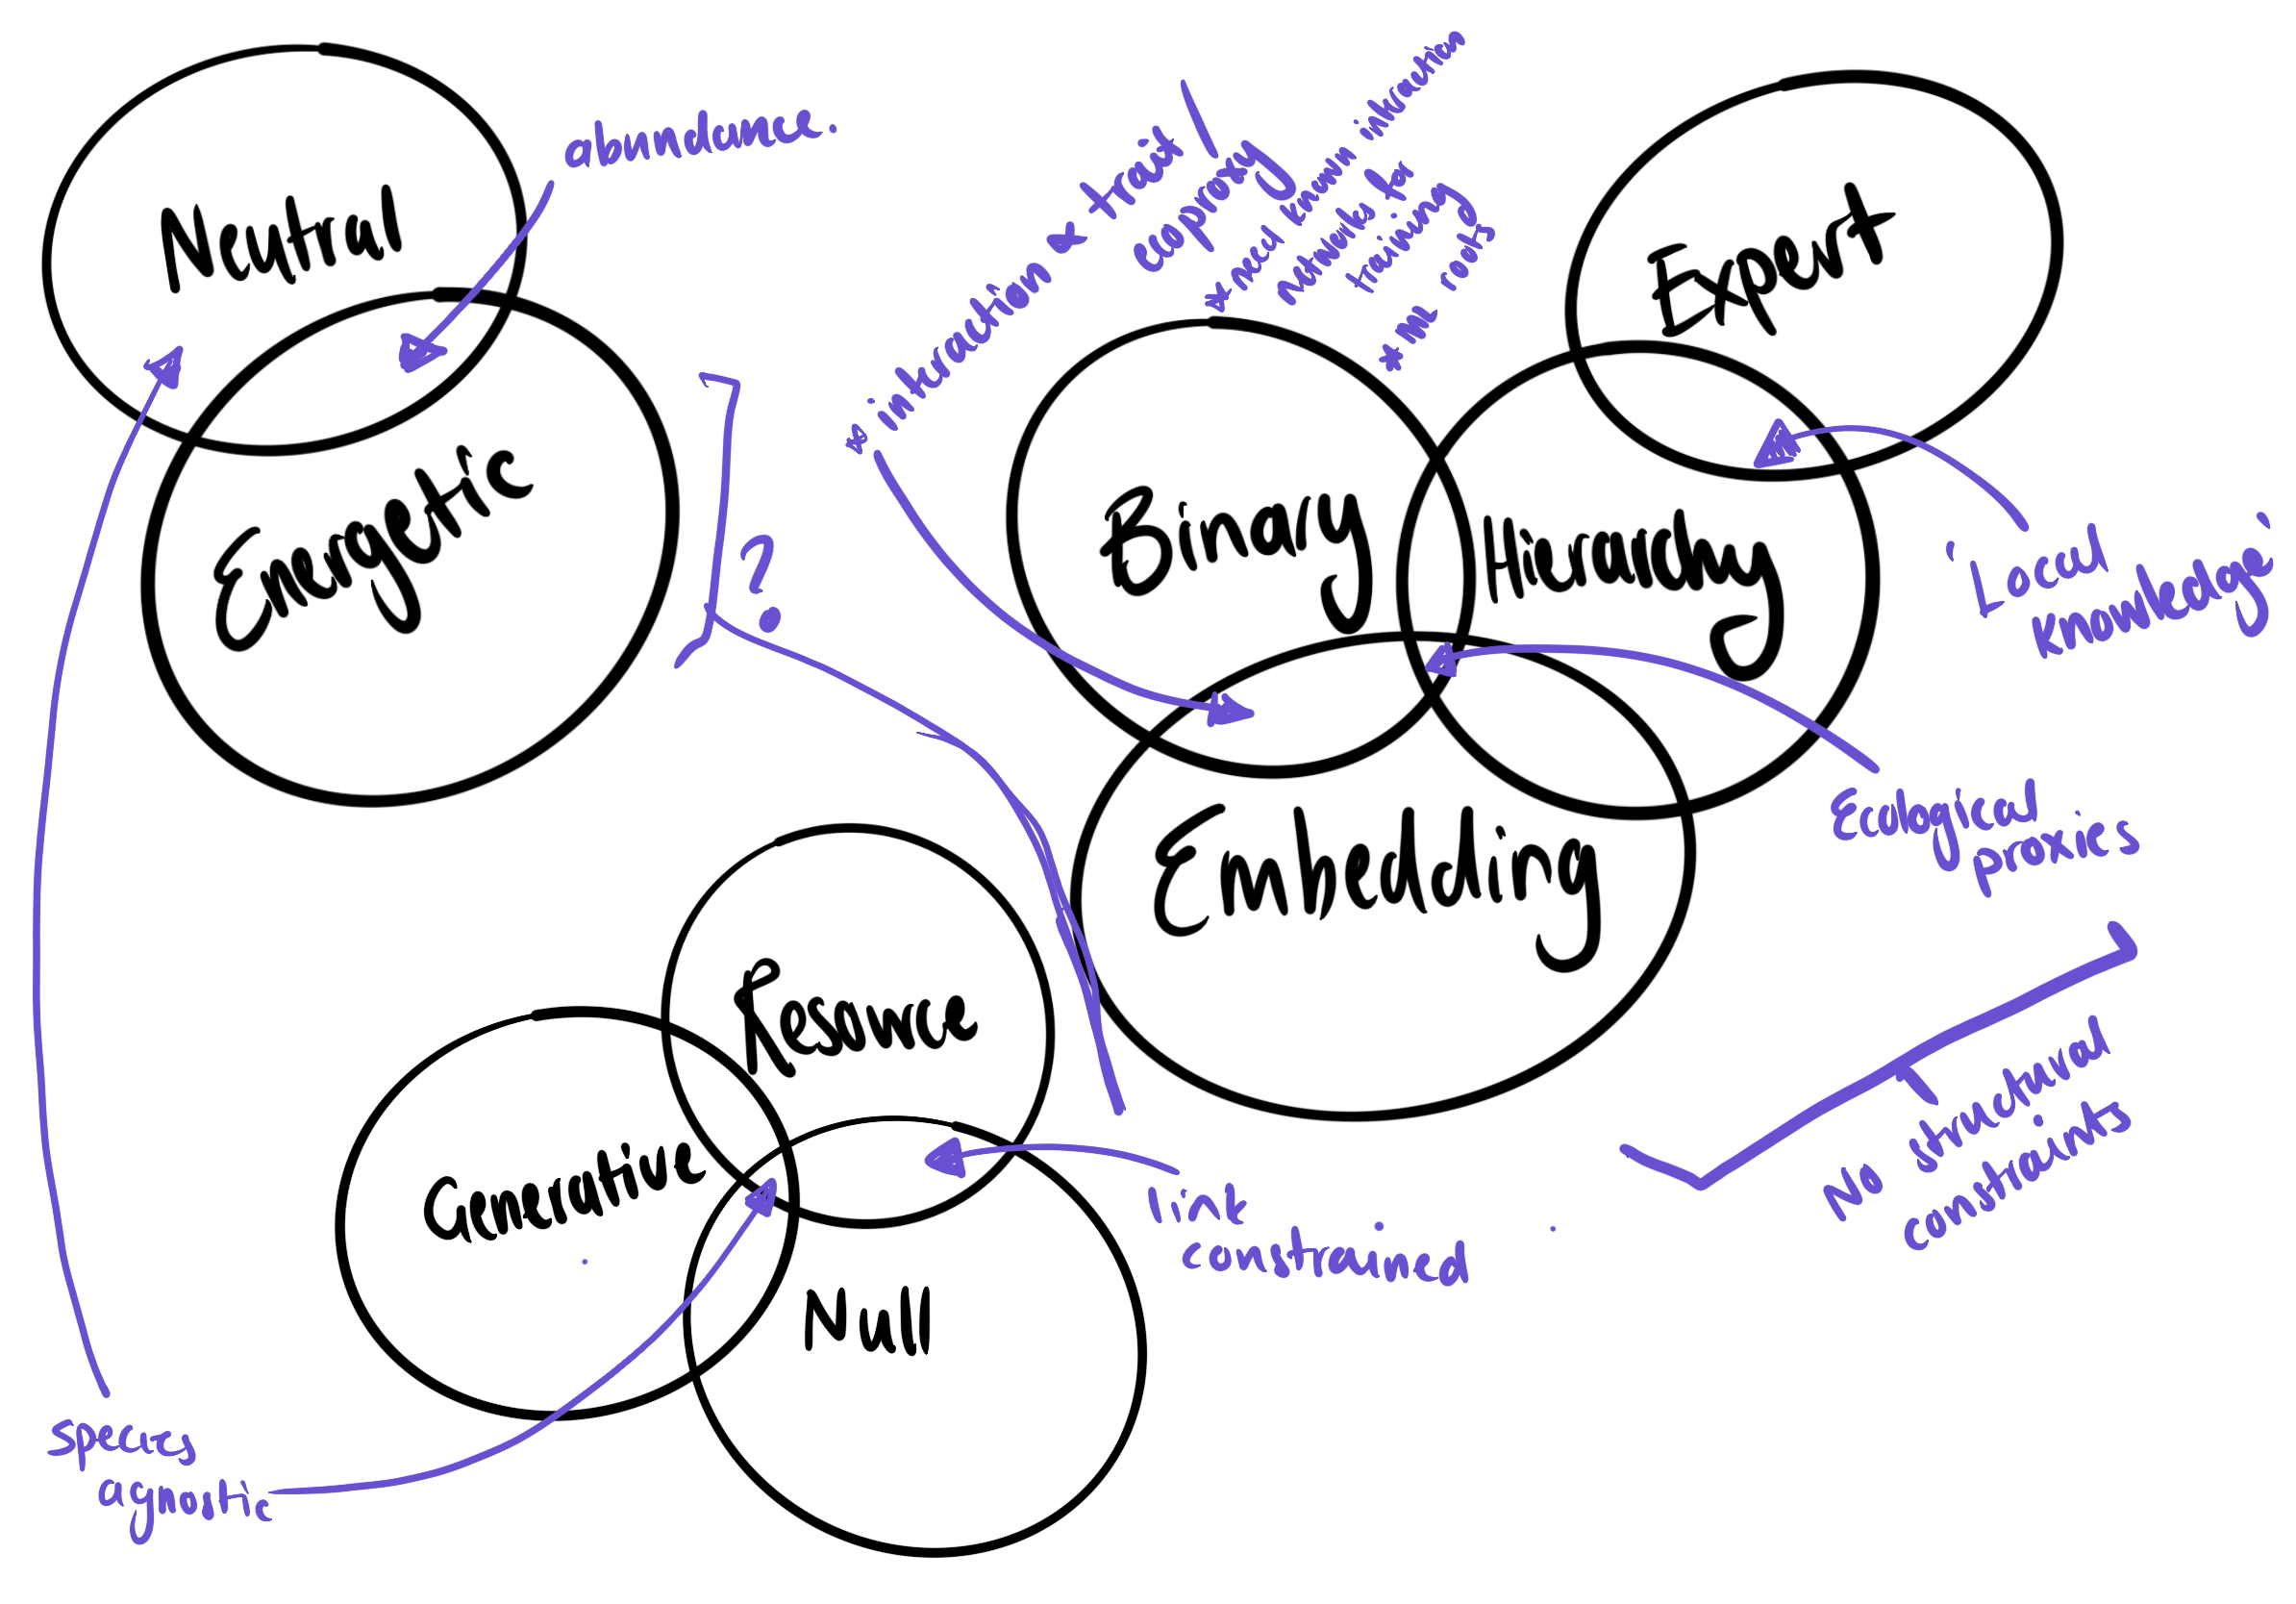
\includegraphics{images/model_venn.png}

}

\caption{\label{fig-venn}I still haven't given up on a sort of venn
diagram idea but maybe it going to be more of a venn-flow chart
hybrid\ldots{}}

\end{figure}%

\begin{figure}

\centering{

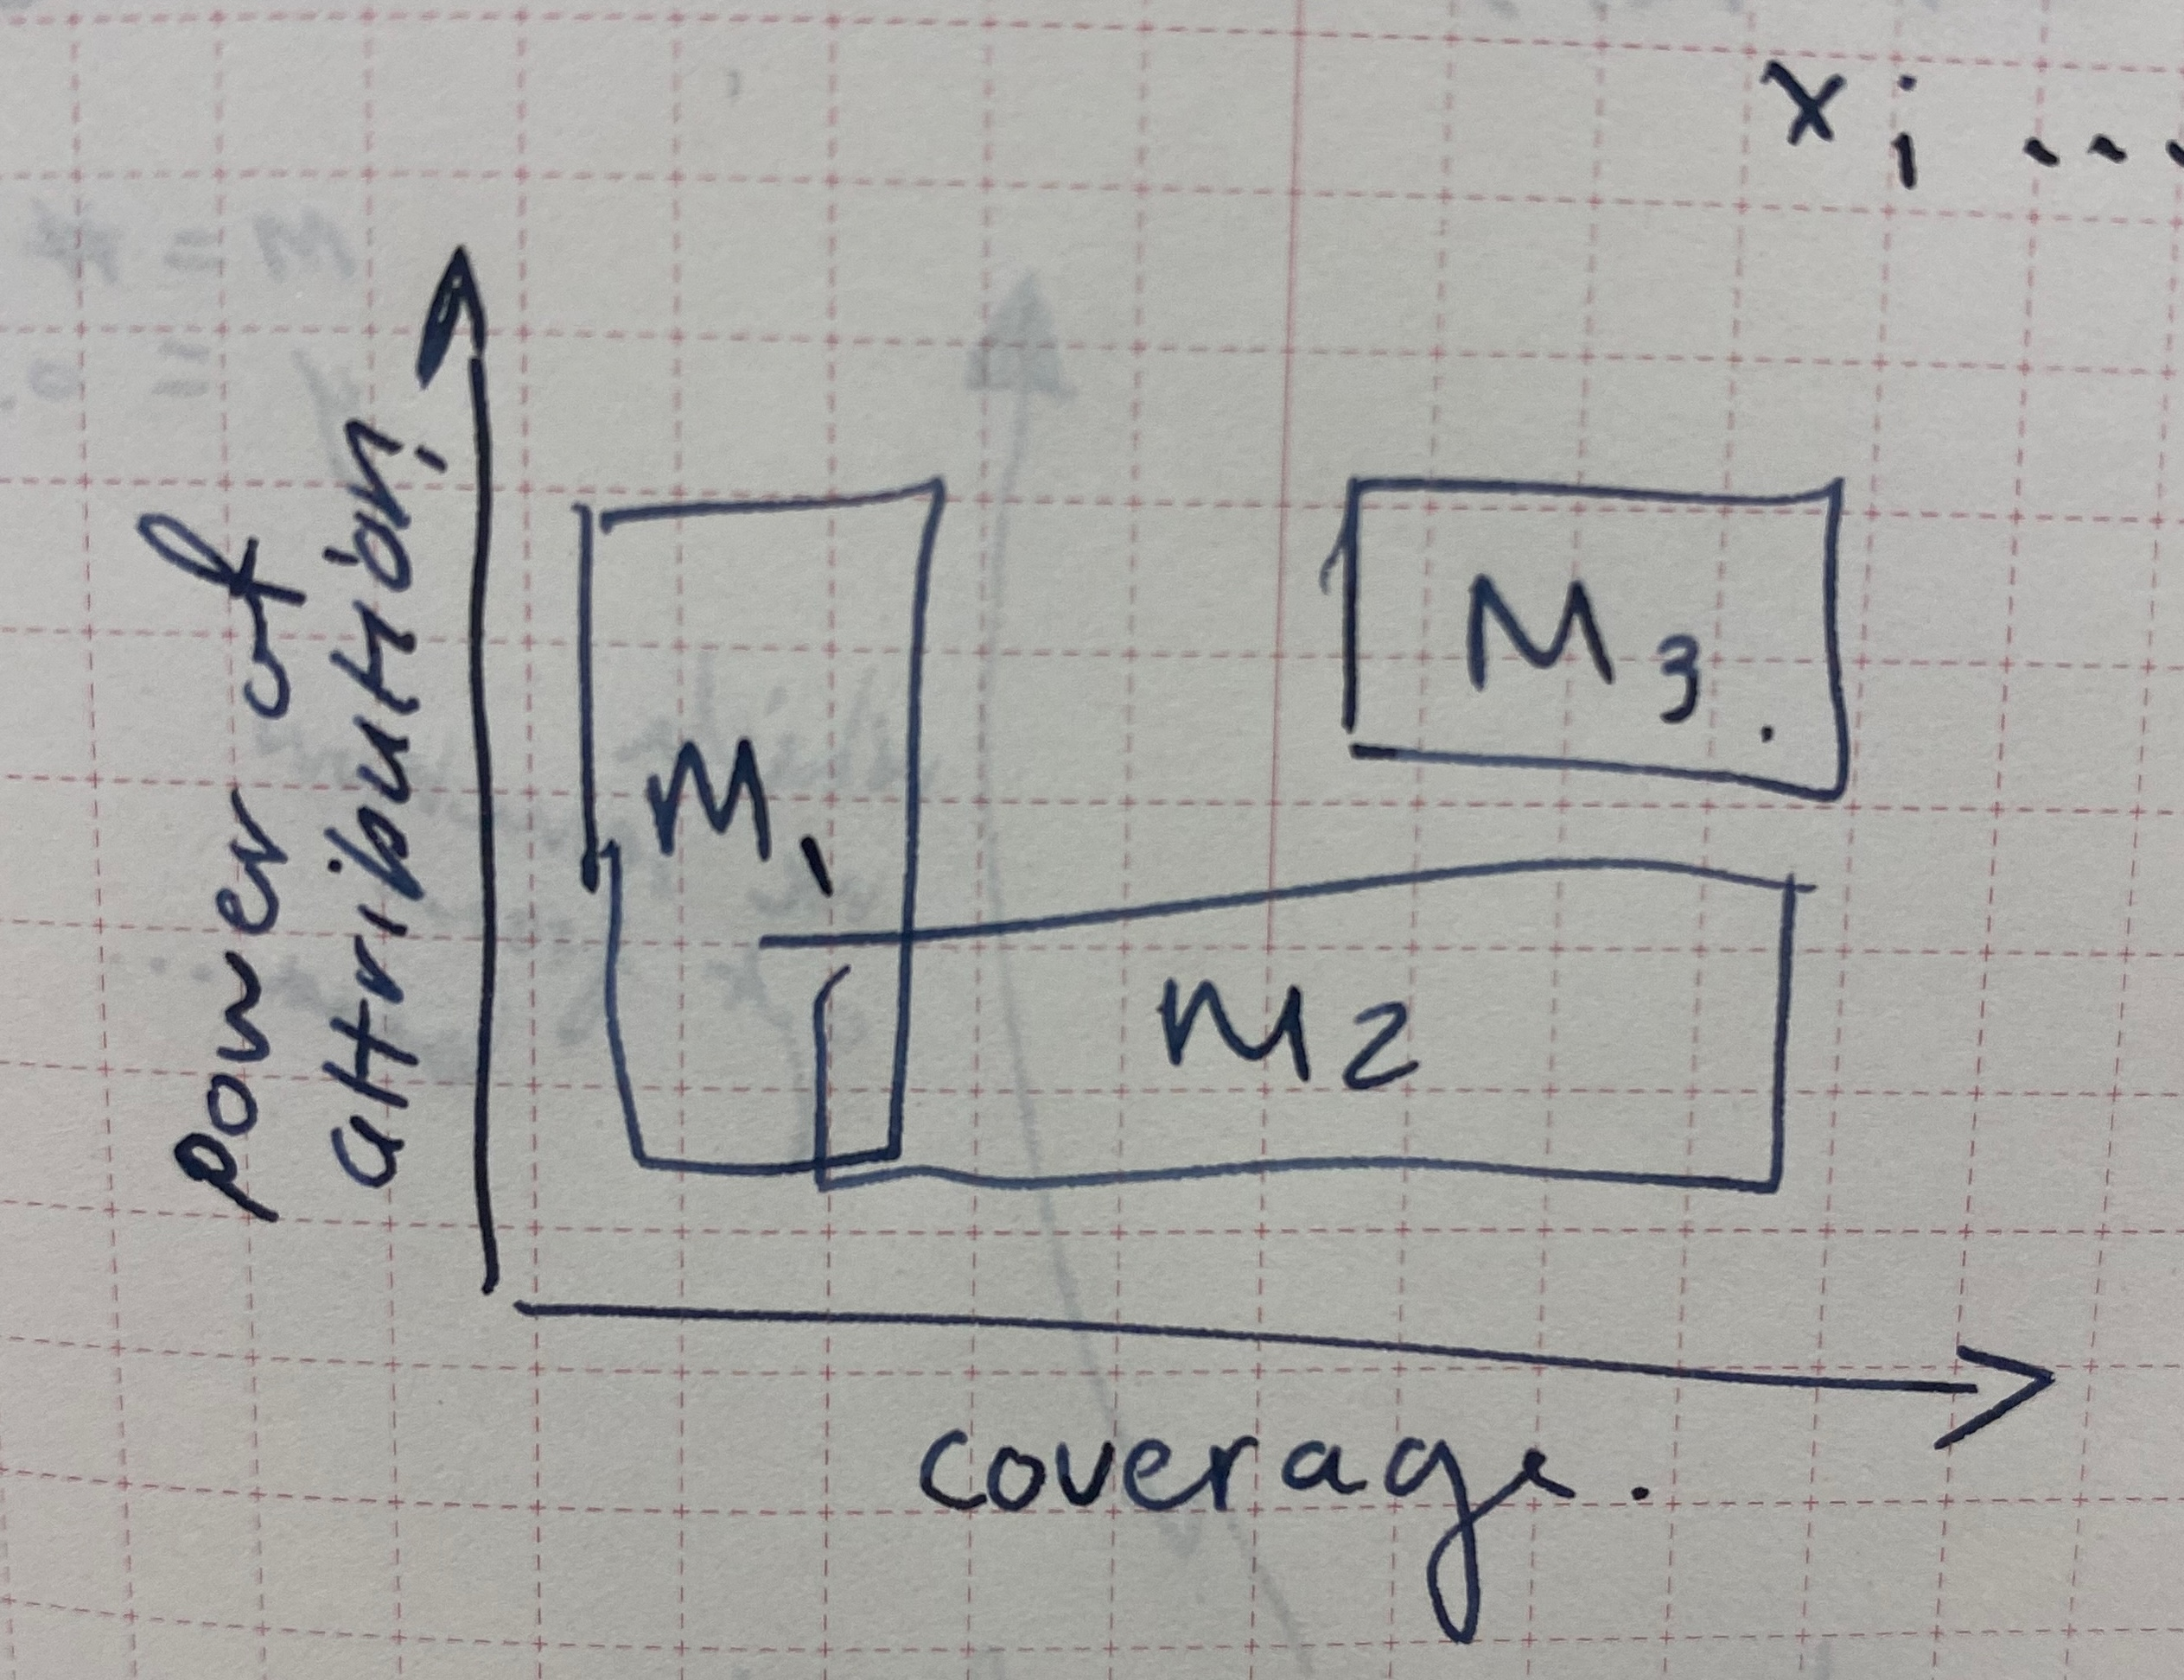
\includegraphics{images/outhwaite_schematic.jpeg}

}

\caption{\label{fig-outhwaite}I like these schematics that Charlie
Outhwaite presented at the EEB seminar (there was a series of them).}

\end{figure}%

\begin{figure}[H]

\centering{

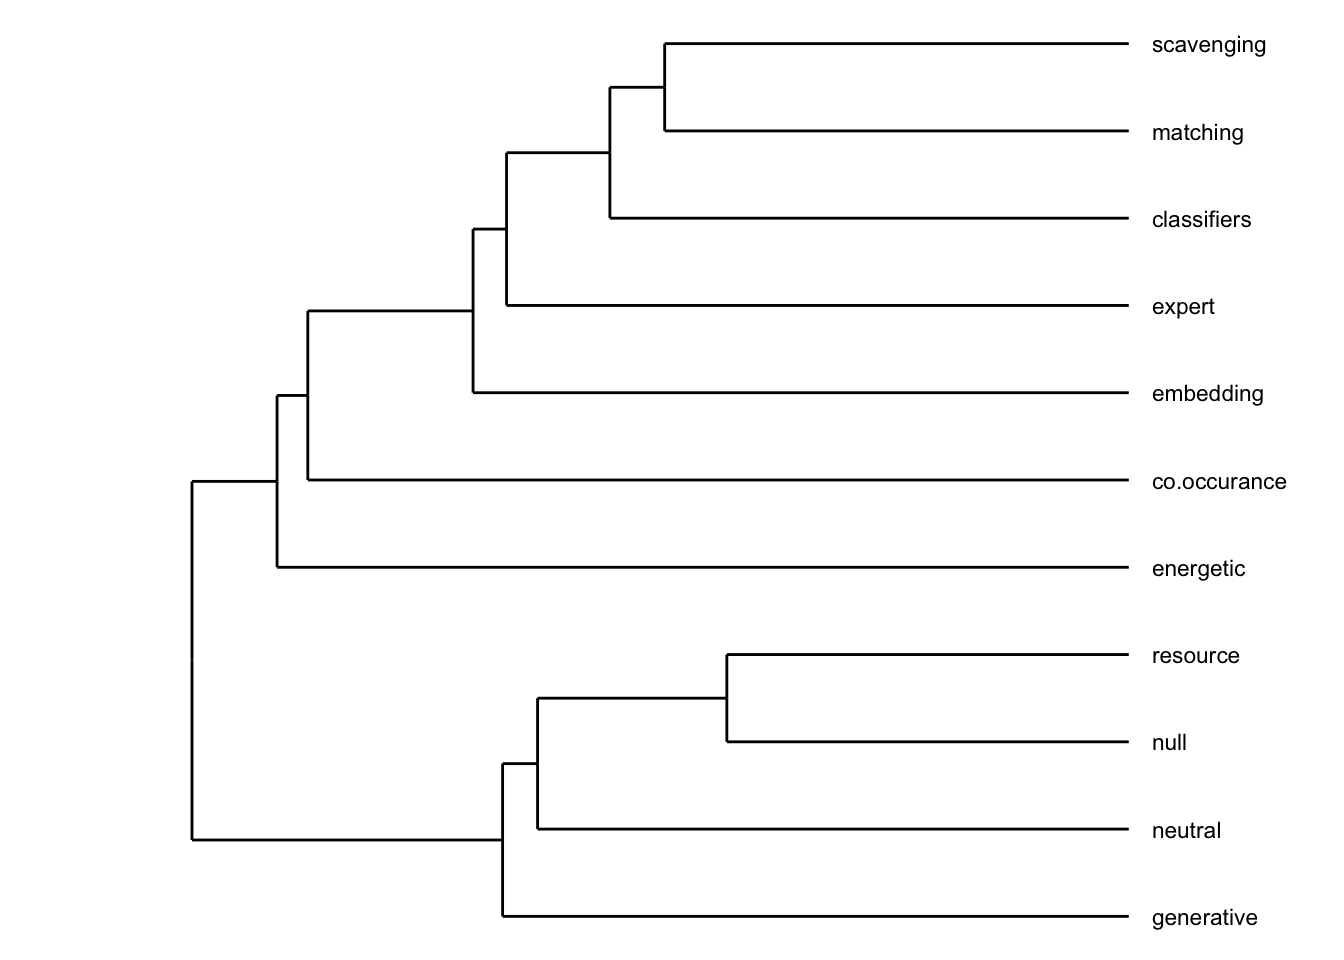
\includegraphics{index_files/figure-latex/notebooks-model_qualitative-fig-dendo-output-1.png}

}

\caption{\label{fig-dendo}Dendrogram of the trait table}

\end{figure}%

\textsubscript{Source:
\href{https://BecksLab.github.io/ms_t_is_for_topology/notebooks/model_qualitative-preview.html\#cell-fig-dendo}{Qualitative
approach to topology generators}}

\subsection{Assessing model outputs}\label{assessing-model-outputs}

Although understanding the underlying philosophy of the different model
families is beneficial it is also important to understand in what
situations the different families are likely to preform well or poorly.
When we are assessing the performance of the different model families it
is beneficial to think of benchmarking these assessments based on two
broader criteria, namely the ability of the model to correctly capture
different elements of the structure of the network and the ability of
the model to correctly retrieve pairwise interactions. When thinking
about how to benchmark models it is perhaps beneficial to take a step
back and once again assess what are the needs of the researcher and
linking this back to what aspects of the network
(Section~\ref{sec-network-anatomy}) are of importance. For example if we
are concerned with being able to successfully predict pairwise
interactions we want to ensure that we are able to retrieve interactions
that really exist but also those that cannot exist (\emph{sensu}
forbidden links Jordano (2016b))

Benchmarking how well a model is doing to capture the desired elements
of a network is also a task that required some thought and
contemplation. Even if we think about the predicting the structure of a
network it is possible that two networks may have the same number of
nodes and links but that those links may be distributed in very
different ways. Thus it is important to think critically about the suite
of summary statistics that are used to assess a model, since there is no
one `silver bullet' summary statistic that will be able to assess if a
model is able to fully replicate an empirical network (Allesina et al.,
2008). One of the main challenges when assessing the ability to retrieve
pairwise interactions is that food webs are sparse (that means that
there are few links given the number of species) and it is important tha
we are able to discern between a model that is able to correctly predict
interactions that do (true positives) and not (true negatives) occur and
one that is simply predicting a lack of interactions (Poisot, 2023).

\begin{quote}
benchmarking requires the use of empirical networks and comparing that
to the predicted one
\end{quote}

\paragraph{Benchmarking for structure}\label{benchmarking-for-structure}

Despite structural models being some of the older model families there
is a distinctive lack of clear guidelines as to how we assess the
ability of these models to replicate the \emph{entire} structure of a
network. In part this may perhaps be driven by the underlying research
agenda and interest in different aspects of capturing the structure of
networks \emph{e.g.,} the obsession with intervality {[}ref{]} or link
distributions {[}ref{]}. However, it is still a good idea to think about
the network in its entirety and to benchmark structural models in a more
holistic manner. Some useful ways to assess how well the model predicts
the shape (\emph{e.g.,} the height (chain length) and\ldots), links
(\emph{e.g.,} connectance), internal structure (\emph{e.g.,} SVD
entropy, Strydom, Dalla Riva, et al. (2021)), and meso-level features
(\emph{e.g.,} motifs, Stouffer et al. (2007)) of a network. This is
shown in Figure~\ref{fig-topology}\ldots{}

\begin{itemize}
\item
  Maybe look at some of the historic papers that compare some of the
  `resource models'
\item
  See also Allesina et al. (2008) and the likelihood function that they
  use for model selection
\item
  Look at Vermaat et al. (2009)
\end{itemize}

\begin{figure}[H]

\centering{

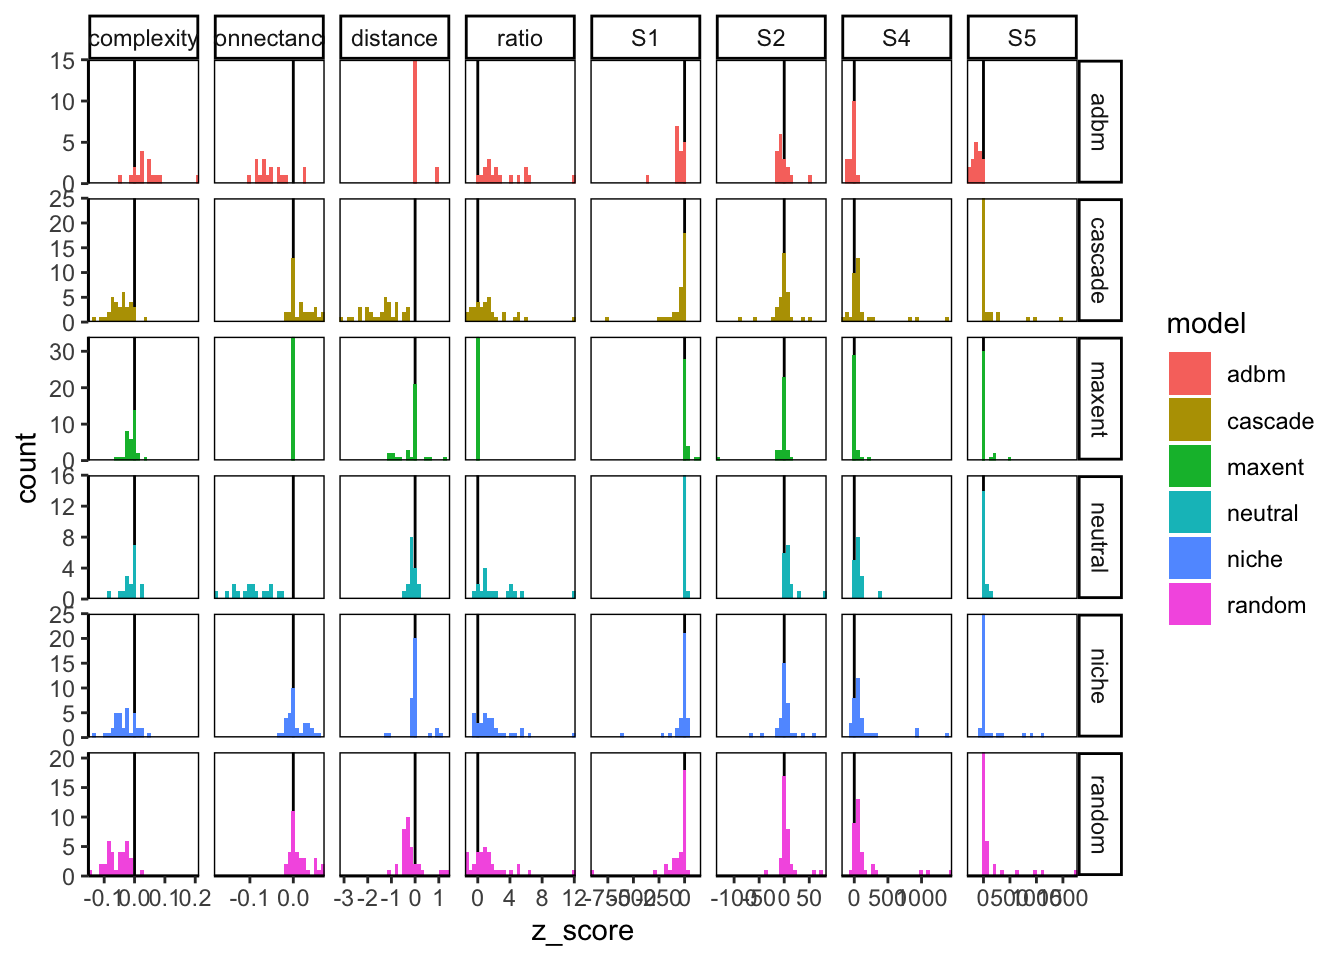
\includegraphics{index_files/figure-latex/notebooks-model_quantitative-fig-topology-output-2.png}

}

\caption{\label{fig-topology}Difference between real and model network
property. S1 - S5 represent the different motif structures identified in
Stouffer et al. (2007).}

\end{figure}%

\textsubscript{Source:
\href{https://BecksLab.github.io/ms_t_is_for_topology/notebooks/model_quantitative-preview.html\#cell-fig-topology}{Quantitative
approach to topology generators}}

\paragraph{Benchmarking for
interactions}\label{benchmarking-for-interactions}

Broadly speaking the task of assessing the ability of a model to predict
interactions as being an assessment of the model's classification
ability (does it correctly predict the presence and absence of
interactions?) and so we want to benchmark the model on how well it is
able to correctly predict these presences and absences. This can be done
in a myriad of ways (Poisot, 2023; Strydom, Catchen, et al., 2021) but
is always based off of the confusion matrix {[}ref maybe?{]}.
Essentially the confusion matrix captures the number of true positives
(interaction predicted as present when it is present), false negatives
(interaction predicted as absent when it is present), false positives
(interaction predicted as present when it is absent), and true negatives
(interaction predicted as absent when it is absent). Using the confusion
matrix it is then possible to assess the `quality' of the model
predictions such as their accuracy or informedness.

As mentioned above one of the main challenges we are faced with when
trying to benchmark interaction predictions is the high class imbalance
(inherit sparsity) of networks, and as highlighted by Poisot (2023) we
can very easy to lull ourselves into a false sense of predictive
accuracy if we use the wrong benchmarking tools --- even a low skill
(fails to predict interactions that are present) model can appear to do
well if we assess it on its ability to correctly predict interactions,
this is because most interactions are absent and so a model that
predicts interactions as being absent will still predict most
interactions correctly. Another aspect of assessing these types of
predictions is quantifying the bias of the model, this will give and
indication id the model tends to systematically over predict one of the
classes. As per Poisot (2023) the best ways to assess the classification
performance of the different models is to use the Precision-Recall
(PR-AUC) to assess precision {[}ref?{]}, and the Matthews correlation
coefficient (MCC) to assess accuracy (Matthews, 1975).

\begin{itemize}
\item
  Caveat regarding the use of real world interaction data both for
  training and validating predictions? \emph{e.g.,} Poisot, Ouellet, et
  al.~et al 2021 and Catchen et al 2023
\item
  ``These results suggest that learning from a dataset with very low
  connectance can be a different task than for more connected networks:
  it becomes increasingly important to capture the mechanisms that make
  an interaction exist, and therefore having a slightly more biased
  training dataset might be beneficial. As connectance increases, the
  need for biased training sets is less prominent, as learning the rules
  for which interactions do not exist starts gaining importance''
\item
  Maybe also looking at how well a model can recover `missing links'
  \emph{i.e.,} false negatives \emph{sensu} what we did in Strydom et
  al. (2022)
\item
  Need to discuss the key differences and implications between
  predicting a metaweb (\emph{sensu} Dunne (2006)) and a network
  realisation. Maybe also Poisot et al. (2015) that discuss how the
  local factors are going to play a role.
\end{itemize}

\begin{figure}

\centering{

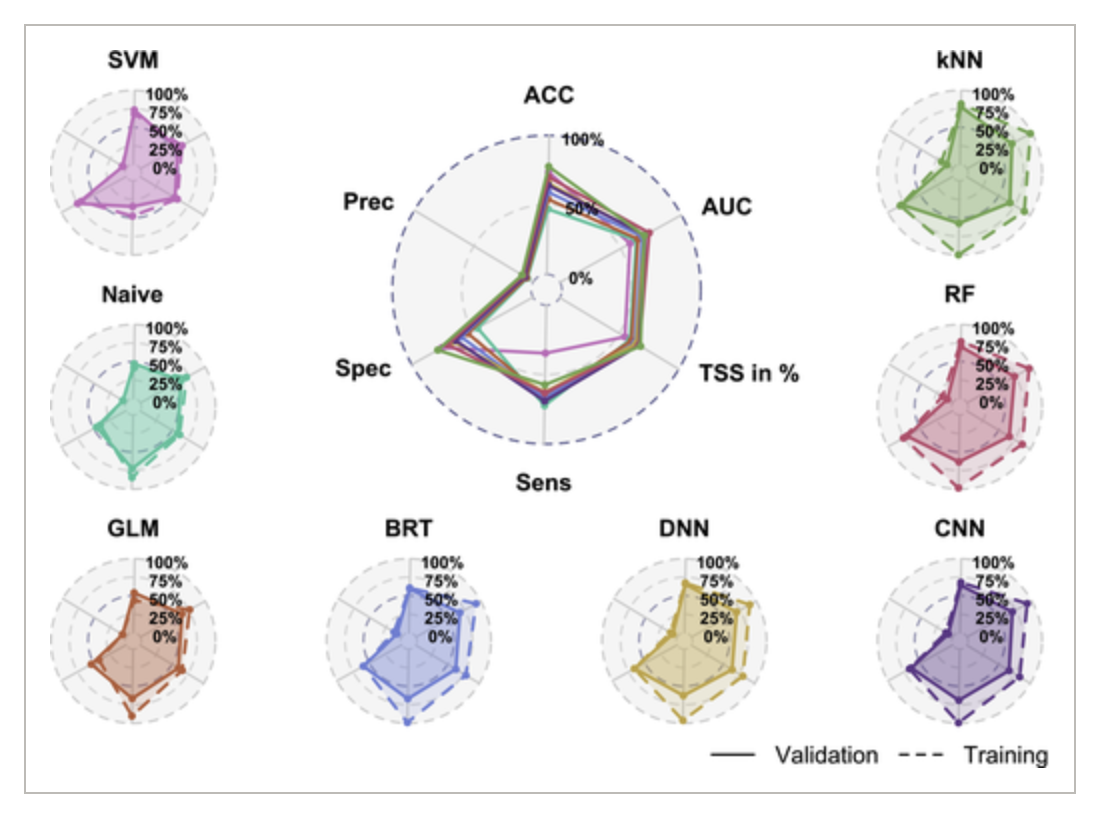
\includegraphics{images/pichler_result.png}

}

\caption{\label{fig-pichler}Moc result from Pichler et al. (2020)}

\end{figure}%

\subsection{The bigger picture}\label{the-bigger-picture}

In addition to thinking about the `performance' if a model it is also
important to be aware of the `unseen' costs and limitations of the
different modelling families. This includes thinking about the need for
additional data sources (such as trait or phylogenetic data), the
computational cost, as well as the time it might take to generate a
network, \emph{e.g.,} binary classifiers require an (often times)
extensive list of additional trait data for the model training process,
which limits predictions to communities for which you do have the
relevant auxiliary data available.

\begin{quote}
What data do I need? Can a make \emph{de novo} predictions? What are the
related `sinks' \emph{e.g.,} computational or time? What does the
network I am constructing actually represent?
\end{quote}

\section{Linking network ecology to the outstanding questions in
ecology}\label{linking-network-ecology-to-the-outstanding-questions-in-ecology}

\begin{itemize}
\item
  Bring up the fact that delimiting a network is in and of itself fuzzy
  - we tend to think of them in terms of snapshots but in reality the
  final (empirical) network is often the result of aggregation over
  multiple timescales.
\item
  Also the fact that \emph{some} people are concerned about the
  taxonomic resolution and cascading effects those might have on our
  understanding of network structure (Pringle, 2020; Pringle \&
  Hutchinson, 2020), we are at risk of losing our ability to distinguish
  the wood from the tree - are we not (at least at times) concerned more
  with understanding ecosystem level processes than with needing to
  understand things \emph{perfectly} at the species level.

  \begin{itemize}
  \tightlist
  \item
    I don't think these `rare'/nuanced links (e.g.~carnivorous hippos)
    are going to rock the boat when we think about networks at the
    structural level. To say this in a different way maybe it comes down
    to thinking about the scale of organisation within a network\ldots{}
    The classical levels of organisation within ecology (population,
    community, \ldots) are also relevant when we think about a networks.
  \end{itemize}
\item
  Brief history of the development of tools within the context of the
  two different fields? Sort of where the theory/body of work was based
  and how that has changed?
\item
  In certain situations structure is `enough' but there may be use cases
  where we are really interested in the node-level interactions
  \emph{i.e.,} species identity is a thing we care about and need to be
  able to retrieve specific interactions at specific nodes correctly.
\item
  What is the purpose of generating a network? Is it an element of a
  bigger question we are asking, \emph{e.g.,} I want to generate a
  series of networks to do some extinction simulations/bioenergetic
  stuff OR are we looking for a `final product' network that is relevant
  to a specific location? (this can still be broad in geographic scope).
\end{itemize}

Interestingly Williams \& Martinez (2008) also explicitly talk about
\emph{structural} food-web models in their introduction\ldots{} so how I
see it that means that there has always been this inherent
acknowledgement that models are functioning at a specific `network
level'.

\begin{quote}
``The resolution of food-web data is demonic because it can radically
change network topology and associated biological inferences in ways
that are unknowable in the absence of better data.'' - Pringle \&
Hutchinson (2020) The counter to this is that structural models are
often not working at the species level and thus the structure remains
`unchanged' when you increase the resolution - I don't think that people
are that concerned with the structure of real world networks barring
connectance and since that scales with species richness anyway your
final proportion will probably still remain the same\ldots{}
\end{quote}

\begin{quote}
``It makes no sense to describe the interaction structure of nodes which
in themselves are poorly defined.'' --- Roslin et al.~(2013, p.~2)
\end{quote}

\section{Discussion}\label{discussion}

\begin{itemize}
\item
  I think a big take home will (hopefully) be how different approaches
  do better in different situations and so you as an end user need to
  take this into consideration and pick accordingly. I think Petchey et
  al. (2011) might have (and share) some thoughts on this (thanks
  Andrew). I feel like I need to look at Berlow et al. (2008) but maybe
  not exactly in this context but vaguely adjacent.
\item
  An interesting thing to also think about (and arguably it will be
  addressed based on some of the other thoughts and ideas) is data
  dependant and data independent `parametrisation' of the models\ldots{}
\item
  Why do interaction models do so badly at predicting structure? Nuance
  of metaweb vs realisation but also time? At the core of it interaction
  models are trained on existing interaction data; this is data that are
  most likely closer to a metaweb than a local realisation even if they
  are being inventoried at a small scale.

  \begin{itemize}
  \tightlist
  \item
    I think this is sort of the crux of the argument presented in
    Brimacombe et al. (2024)
  \end{itemize}
\end{itemize}

\begin{quote}
\emph{``we highlight an interesting paradox: the models with the best
performance measures are not necessarily the models with the closest
reconstructed network structure.''} - Poisot (2023)
\end{quote}

\begin{itemize}
\item
  \emph{Do we need network models to predict interactions and
  interaction models to predict structure?} (lets not think about that
  too hard or I might just have to sit in silence for a while\ldots)

  \begin{itemize}
  \item
    ``Another argument for the joint prediction of networks and
    interactions is to reduce circularity and biases in the predictions.
    As an example, models like linear filtering generate probabilities
    of non-observed interactions existing, but do so based on measured
    network properties.'' - Strydom, Catchen, et al. (2021)
  \item
    Aligning (dove-tailing) with this the idea of ensemble modelling as
    presented by Becker et al. (2022)
  \end{itemize}
\item
  It will be interesting to bring up the idea that if a model is missing
  a specific pairwise link but doing well at the structural level then
  when does it matter?
\item
  Close out with a call to action that we have models that predict
  networks very well and models that predict interactions very well but
  nothing that is doing well at predicting both - this is where we
  should be focusing our attention when it comes to furthering model
  development. (we need models that will fill the space in the top right
  quadrant of panel A in Figure~\ref{fig-concept})
\end{itemize}

\subsection{Downsampling}\label{downsampling}

\begin{itemize}
\item
  Dansereau et al. (2023)
\item
  ``That being said, there is a compelling argument for the need to
  `combine' these smaller functional units with larger spatial networks
  (Fortin et al., 2021) and that we should also start thinking about the
  interplay of time and space (Estay et al., 2023). Although deciding
  exactly what measure might actually be driving differences between
  local networks and the regional metaweb might not be that simple
  (Saravia et al., 2022).''
\end{itemize}

\section*{References}\label{references}
\addcontentsline{toc}{section}{References}

\phantomsection\label{refs}
\begin{CSLReferences}{1}{0}
\bibitem[\citeproctext]{ref-allesinaGeneralModelFood2008}
Allesina, S., Alonso, D., \& Pascual, M. (2008). A {General Model} for
{Food Web Structure}. \emph{Science}, \emph{320}(5876), 658--661.
\url{https://doi.org/10.1126/science.1156269}

\bibitem[\citeproctext]{ref-banvilleWhatConstrainsFood2023}
Banville, F., Gravel, D., \& Poisot, T. (2023). What constrains food
webs? {A} maximum entropy framework for predicting their structure with
minimal biases. \emph{PLOS Computational Biology}, \emph{19}(9),
e1011458. \url{https://doi.org/10.1371/journal.pcbi.1011458}

\bibitem[\citeproctext]{ref-bascompteNestedAssemblyPlantanimal2003}
Bascompte, J., Jordano, P., Melian, C. J., \& Olesen, J. M. (2003). The
nested assembly of plant-animal mutualistic networks. \emph{Proceedings
of the National Academy of Sciences}, \emph{100}(16), 9383--9387.
\url{https://doi.org/10.1073/pnas.1633576100}

\bibitem[\citeproctext]{ref-beckerOptimisingPredictiveModels2022}
Becker, D. J., Albery, G. F., Sjodin, A. R., Poisot, T., Bergner, L. M.,
Chen, B., Cohen, L. E., Dallas, T. A., Eskew, E. A., Fagre, A. C.,
Farrell, M. J., Guth, S., Han, B. A., Simmons, N. B., Stock, M.,
Teeling, E. C., \& Carlson, C. J. (2022). Optimising predictive models
to prioritise viral discovery in zoonotic reservoirs. \emph{The Lancet
Microbe}, \emph{3}(8), e625--e637.
\url{https://doi.org/10.1016/S2666-5247(21)00245-7}

\bibitem[\citeproctext]{ref-beckermanForagingBiologyPredicts2006}
Beckerman, A. P., Petchey, O. L., \& Warren, P. H. (2006). Foraging
biology predicts food web complexity. \emph{Proceedings of the National
Academy of Sciences}, \emph{103}(37), 13745--13749.
\url{https://doi.org/10.1073/pnas.0603039103}

\bibitem[\citeproctext]{ref-berlowGoldilocksFactorFood2008}
Berlow, E. L., Brose, U., \& Martinez, N. D. (2008). The {``{Goldilocks}
factor''} in food webs. \emph{Proceedings of the National Academy of
Sciences}, \emph{105}(11), 4079--4080.
\url{https://doi.org/10.1073/pnas.0800967105}

\bibitem[\citeproctext]{ref-berlowInteractionStrengthsFood2004}
Berlow, E. L., Neutel, A.-M., Cohen, J. E., de Ruiter, P. C., Ebenman,
B., Emmerson, M., Fox, J. W., Jansen, V. A. A., Iwan Jones, J.,
Kokkoris, G. D., Logofet, D. O., McKane, A. J., Montoya, J. M., \&
Petchey, O. (2004). Interaction strengths in food webs: Issues and
opportunities. \emph{Journal of Animal Ecology}, \emph{73}(3), 585--598.
\url{https://doi.org/10.1111/j.0021-8790.2004.00833.x}

\bibitem[\citeproctext]{ref-bhatiaNetworkbasedRestorationStrategies2023}
Bhatia, U., Dubey, S., Gouhier, T. C., \& Ganguly, A. R. (2023).
Network-based restoration strategies maximize ecosystem recovery.
\emph{Communications Biology}, \emph{6}(1), 1--10.
\url{https://doi.org/10.1038/s42003-023-05622-3}

\bibitem[\citeproctext]{ref-blanchetCooccurrenceNotEvidence2020}
Blanchet, F. G., Cazelles, K., \& Gravel, D. (2020). Co-occurrence is
not evidence of ecological interactions. \emph{Ecology Letters},
\emph{23}(7), 1050--1063. \url{https://doi.org/10.1111/ele.13525}

\bibitem[\citeproctext]{ref-brimacombeApplyingMethodIts2024}
Brimacombe, C., Bodner, K., \& Fortin, M.-J. (2024). \emph{Applying a
method before its proof-of-concept: {A} cautionary tale using inferred
food webs}. \url{https://doi.org/10.13140/RG.2.2.22076.65927}

\bibitem[\citeproctext]{ref-brimacombeShortcomingsReusingSpecies2023}
Brimacombe, C., Bodner, K., Michalska-Smith, M., Poisot, T., \& Fortin,
M.-J. (2023). Shortcomings of reusing species interaction networks
created by different sets of researchers. \emph{PLOS Biology},
\emph{21}(4), e3002068.
\url{https://doi.org/10.1371/journal.pbio.3002068}

\bibitem[\citeproctext]{ref-caronAddressingEltonianShortfall2022}
Caron, D., Maiorano, L., Thuiller, W., \& Pollock, L. J. (2022).
Addressing the {Eltonian} shortfall with trait-based interaction models.
\emph{Ecology Letters}, \emph{25}(4), 889--899.
\url{https://doi.org/10.1111/ele.13966}

\bibitem[\citeproctext]{ref-cattinPhylogeneticConstraintsAdaptation2004}
Cattin, M.-F., Bersier, L.-F., Banašek-Richter, C., Baltensperger, R.,
\& Gabriel, J.-P. (2004). Phylogenetic constraints and adaptation
explain food-web structure. \emph{Nature}, \emph{427}(6977), 835--839.
\url{https://doi.org/10.1038/nature02327}

\bibitem[\citeproctext]{ref-cirtwillQuantitativeFrameworkInvestigating2019}
Cirtwill, A. R., Eklf, A., Roslin, T., Wootton, K., \& Gravel, D.
(2019). A quantitative framework for investigating the reliability of
empirical network construction. \emph{Methods in Ecology and Evolution},
\emph{0}(ja). \url{https://doi.org/10.1111/2041-210X.13180}

\bibitem[\citeproctext]{ref-cohenFoodWebsDimensionality1977}
Cohen, J. E. (1977). Food webs and the dimensionality of trophic niche
space. \emph{Proceedings of the National Academy of Sciences},
\emph{74}(10), 4533--4536. \url{https://doi.org/10.1073/pnas.74.10.4533}

\bibitem[\citeproctext]{ref-cohenCommunityFoodWebs1990}
Cohen, J. E., Briand, F., \& Newman, C. (1990). \emph{Community {Food
Webs}: {Data} and {Theory}}. Springer-Verlag.

\bibitem[\citeproctext]{ref-cohenStochasticTheoryCommunity1985}
Cohen, J. E., Newman, C. M., \& Steele, J. H. (1985). A stochastic
theory of community food webs {I}. {Models} and aggregated data.
\emph{Proceedings of the Royal Society of London. Series B. Biological
Sciences}, \emph{224}(1237), 421--448.
\url{https://doi.org/10.1098/rspb.1985.0042}

\bibitem[\citeproctext]{ref-daleGraphsSpatialGraphs2010}
Dale, M. R. T., \& Fortin, M.-J. (2010). From {Graphs} to {Spatial
Graphs}. \emph{Annual Review of Ecology, Evolution, and Systematics},
\emph{41}, 21--38. \url{https://www.jstor.org/stable/27896212}

\bibitem[\citeproctext]{ref-dansereauSpatiallyExplicitPredictions2023}
Dansereau, G., Barros, C., \& Poisot, T. (2023). \emph{Spatially
explicit predictions of food web structure from regional level data}.

\bibitem[\citeproctext]{ref-darwinOriginSpeciesMeans1859}
Darwin, C. (1859). \emph{On the {Origin} of {Species} by {Means} of
{Natural Selection}, or the {Preservation} of {Favoured Races} in the
{Struggle} for {Life}}. J. Murray.

\bibitem[\citeproctext]{ref-deangelisModelTropicInteraction1975}
DeAngelis, D. L., Goldstein, R. A., \& O'Neill, R. V. (1975). A {Model}
for {Tropic Interaction}. \emph{Ecology}, \emph{56}(4), 881--892.
\url{https://doi.org/10.2307/1936298}

\bibitem[\citeproctext]{ref-delmasAnalysingEcologicalNetworks2019}
Delmas, E., Besson, M., Brice, M.-H., Burkle, L. A., Riva, G. V. D.,
Fortin, M.-J., Gravel, D., Guimarães, P. R., Hembry, D. H., Newman, E.
A., Olesen, J. M., Pires, M. M., Yeakel, J. D., \& Poisot, T. (2019).
Analysing ecological networks of species interactions. \emph{Biological
Reviews}, \emph{94}(1), 16--36. \url{https://doi.org/10.1111/brv.12433}

\bibitem[\citeproctext]{ref-desjardins-proulxEcologicalInteractionsNetflix2017}
Desjardins-Proulx, P., Laigle, I., Poisot, T., \& Gravel, D. (2017).
Ecological interactions and the {Netflix} problem. \emph{PeerJ},
\emph{5}, e3644. \url{https://doi.org/10.7717/peerj.3644}

\bibitem[\citeproctext]{ref-dunneNetworkStructureFood2006}
Dunne, J. A. (2006). The {Network Structure} of {Food Webs}. In J. A.
Dunne \& M. Pascual (Eds.), \emph{Ecological networks: {Linking}
structure and dynamics} (pp. 27--86). Oxford University Press.

\bibitem[\citeproctext]{ref-dunneCompilationNetworkAnalyses2008}
Dunne, J. A., Williams, R. J., Martinez, N. D., Wood, R. A., \& Erwin,
D. H. (2008). Compilation and {Network Analyses} of {Cambrian Food
Webs}. \emph{PLOS Biology}, \emph{6}(4), e102.
\url{https://doi.org/10.1371/journal.pbio.0060102}

\bibitem[\citeproctext]{ref-eklofSecondaryExtinctionsFood2013}
Eklöf, A., Tang, S., \& Allesina, S. (2013). Secondary extinctions in
food webs: A {Bayesian} network approach. \emph{Methods in Ecology and
Evolution}, \emph{4}(8), 760--770.
\url{https://doi.org/10.1111/2041-210X.12062}

\bibitem[\citeproctext]{ref-estayEditorialPatternsProcesses2023}
Estay, S. A., Fortin, M.-J., \& López, D. N. (2023). Editorial:
{Patterns} and processes in ecological networks over space.
\emph{Frontiers in Ecology and Evolution}, \emph{11}.

\bibitem[\citeproctext]{ref-fortinNetworkEcologyDynamic2021}
Fortin, M.-J., Dale, M. R. T., \& Brimacombe, C. (2021). Network ecology
in dynamic landscapes. \emph{Proceedings of the Royal Society B:
Biological Sciences}, \emph{288}(1949), rspb.2020.1889, 20201889.
\url{https://doi.org/10.1098/rspb.2020.1889}

\bibitem[\citeproctext]{ref-fortinSpatialStatisticsSpatial2012}
Fortin, M.-J., James, P. M. A., MacKenzie, A., Melles, S. J., \&
Rayfield, B. (2012). Spatial statistics, spatial regression, and graph
theory in ecology. \emph{Spatial Statistics}, \emph{1}, 100--109.
\url{https://doi.org/10.1016/j.spasta.2012.02.004}

\bibitem[\citeproctext]{ref-fortunaHabitatLossStructure2006}
Fortuna, M. A., \& Bascompte, J. (2006). Habitat loss and the structure
of plant-animal mutualistic networks: {Mutualistic} networks and habitat
loss. \emph{Ecology Letters}, \emph{9}(3), 281--286.
\url{https://doi.org/10.1111/j.1461-0248.2005.00868.x}

\bibitem[\citeproctext]{ref-gravelInferringFoodWeb2013}
Gravel, D., Poisot, T., Albouy, C., Velez, L., \& Mouillot, D. (2013).
Inferring food web structure from predator--prey body size
relationships. \emph{Methods in Ecology and Evolution}, \emph{4}(11),
1083--1090. \url{https://doi.org/10.1111/2041-210X.12103}

\bibitem[\citeproctext]{ref-grayJoiningDotsAutomated2015}
Gray, C., Figueroa, D. H., Hudson, L. N., Ma, A., Perkins, D., \&
Woodward, G. (2015). Joining the dots: {An} automated method for
constructing food webs from compendia of published interactions.
\emph{Food Webs}, \emph{5}, 11--20.
\url{https://doi.org/10.1016/j.fooweb.2015.09.001}

\bibitem[\citeproctext]{ref-jordanoChasingEcologicalInteractions2016}
Jordano, P. (2016a). Chasing {Ecological Interactions}. \emph{PLOS
Biology}, \emph{14}(9), e1002559.
\url{https://doi.org/10.1371/journal.pbio.1002559}

\bibitem[\citeproctext]{ref-jordanoSamplingNetworksEcological2016}
Jordano, P. (2016b). Sampling networks of ecological interactions.
\emph{Functional Ecology}. \url{https://doi.org/10.1111/1365-2435.12763}

\bibitem[\citeproctext]{ref-llewelynPredictingPredatorPrey2023}
Llewelyn, J., Strona, G., Dickman, C. R., Greenville, A. C., Wardle, G.
M., Lee, M. S. Y., Doherty, S., Shabani, F., Saltré, F., \& Bradshaw, C.
J. A. (2023). Predicting predator--prey interactions in terrestrial
endotherms using random forest. \emph{Ecography}, \emph{2023}(9),
e06619. \url{https://doi.org/10.1111/ecog.06619}

\bibitem[\citeproctext]{ref-maioranoTETRAEUSpecieslevelTrophic2020}
Maiorano, L., Montemaggiori, A., Ficetola, G. F., O'Connor, L., \&
Thuiller, W. (2020). {TETRA-EU} 1.0: {A} species-level trophic metaweb
of {European} tetrapods. \emph{Global Ecology and Biogeography},
\emph{29}(9), 1452--1457. \url{https://doi.org/10.1111/geb.13138}

\bibitem[\citeproctext]{ref-matthewsComparisonPredictedObserved1975}
Matthews, B. W. (1975). Comparison of the predicted and observed
secondary structure of {T4} phage lysozyme. \emph{Biochimica Et
Biophysica Acta (BBA) - Protein Structure}, \emph{405}(2), 442--451.
\url{https://doi.org/10.1016/0005-2795(75)90109-9}

\bibitem[\citeproctext]{ref-morales-castillaInferringBioticInteractions2015}
Morales-Castilla, I., Matias, M. G., Gravel, D., \& Araújo, M. B.
(2015). Inferring biotic interactions from proxies. \emph{Trends in
Ecology \& Evolution}, \emph{30}(6), 347--356.
\url{https://doi.org/10.1016/j.tree.2015.03.014}

\bibitem[\citeproctext]{ref-ohlmannMappingImprintBiotic2018}
Ohlmann, M., Mazel, F., Chalmandrier, L., Bec, S., Coissac, E., Gielly,
L., Pansu, J., Schilling, V., Taberlet, P., Zinger, L., Chave, J., \&
Thuiller, W. (2018). Mapping the imprint of biotic interactions on
{\(\beta\)}-diversity. \emph{Ecology Letters}, \emph{21}(11),
1660--1669. \url{https://doi.org/10.1111/ele.13143}

\bibitem[\citeproctext]{ref-petcheySizeForagingFood2008}
Petchey, O. L., Beckerman, A. P., Riede, J. O., \& Warren, P. H. (2008).
Size, foraging, and food web structure. \emph{Proceedings of the
National Academy of Sciences}, \emph{105}(11), 4191--4196.
\url{https://doi.org/10.1073/pnas.0710672105}

\bibitem[\citeproctext]{ref-petcheyFitEfficiencyBiology2011}
Petchey, O. L., Beckerman, A. P., Riede, J. O., \& Warren, P. H. (2011).
Fit, efficiency, and biology: {Some} thoughts on judging food web
models. \emph{Journal of Theoretical Biology}, \emph{279}(1), 169--171.
\url{https://doi.org/10.1016/j.jtbi.2011.03.019}

\bibitem[\citeproctext]{ref-pichlerMachineLearningAlgorithms2020}
Pichler, M., Boreux, V., Klein, A.-M., Schleuning, M., \& Hartig, F.
(2020). Machine learning algorithms to infer trait-matching and predict
species interactions in ecological networks. \emph{Methods in Ecology
and Evolution}, \emph{11}(2), 281--293.
\url{https://doi.org/10.1111/2041-210X.13329}

\bibitem[\citeproctext]{ref-poelenGlobalBioticInteractions2014}
Poelen, J. H., Simons, J. D., \& Mungall, C. J. (2014). Global biotic
interactions: {An} open infrastructure to share and analyze
species-interaction datasets. \emph{Ecological Informatics}, \emph{24},
148--159. \url{https://doi.org/10.1016/j.ecoinf.2014.08.005}

\bibitem[\citeproctext]{ref-poisotGuidelinesPredictionSpecies2023}
Poisot, T. (2023). Guidelines for the prediction of species interactions
through binary classification. \emph{Methods in Ecology and Evolution},
\emph{14}(5), 1333--1345. \url{https://doi.org/10.1111/2041-210X.14071}

\bibitem[\citeproctext]{ref-poisotMangalMakingEcological2016}
Poisot, T., Baiser, B., Dunne, J., Kéfi, S., Massol, F., Mouquet, N.,
Romanuk, T. N., Stouffer, D. B., Wood, S. A., \& Gravel, D. (2016).
Mangal -- making ecological network analysis simple. \emph{Ecography},
\emph{39}(4), 384--390. \url{https://doi.org/10.1111/ecog.00976}

\bibitem[\citeproctext]{ref-poisotGlobalKnowledgeGaps2021}
Poisot, T., Bergeron, G., Cazelles, K., Dallas, T., Gravel, D.,
MacDonald, A., Mercier, B., Violet, C., \& Vissault, S. (2021). Global
knowledge gaps in species interaction networks data. \emph{Journal of
Biogeography}, \emph{n/a}(n/a). \url{https://doi.org/10.1111/jbi.14127}

\bibitem[\citeproctext]{ref-poisotStructureProbabilisticNetworks2016}
Poisot, T., Cirtwill, A., Cazelles, K., Gravel, D., Fortin, M.-J., \&
Stouffer, D. (2016). The structure of probabilistic networks.
\emph{Methods in Ecology and Evolution}, \emph{7}(3), 303--312.
\url{https://doi.org/10}

\bibitem[\citeproctext]{ref-poisotSyntheticDatasetsCommunity2016}
Poisot, T., Gravel, D., Leroux, S., Wood, S. A., Fortin, M.-J., Baiser,
B., Cirtwill, A. R., Araújo, M. B., \& Stouffer, D. B. (2016). Synthetic
datasets and community tools for the rapid testing of ecological
hypotheses. \emph{Ecography}, \emph{39}(4), 402--408.
\url{https://doi.org/10.1111/ecog.01941}

\bibitem[\citeproctext]{ref-poisotSpeciesWhyEcological2015}
Poisot, T., Stouffer, D. B., \& Gravel, D. (2015). Beyond species: Why
ecological interaction networks vary through space and time.
\emph{Oikos}, \emph{124}(3), 243--251.
\url{https://doi.org/10.1111/oik.01719}

\bibitem[\citeproctext]{ref-poisotDescribeUnderstandPredict2016}
Poisot, T., Stouffer, D. B., \& Kéfi, S. (2016). Describe, understand
and predict: Why do we need networks in ecology? \emph{Functional
Ecology}, \emph{30}(12), 1878--1882.
\url{https://www.jstor.org/stable/48582345}

\bibitem[\citeproctext]{ref-pomeranzInferringPredatorPrey2019}
Pomeranz, J. P. F., Thompson, R. M., Poisot, T., \& Harding, J. S.
(2019). Inferring predator--prey interactions in food webs.
\emph{Methods in Ecology and Evolution}, \emph{10}(3), 356--367.
\url{https://doi.org/10.1111/2041-210X.13125}

\bibitem[\citeproctext]{ref-pringleUntanglingFoodWebs2020}
Pringle, R. M. (2020). Untangling {Food Webs}. In \emph{Untangling {Food
Webs}} (pp. 225--238). Princeton University Press.
\url{https://doi.org/10.1515/9780691195322-020}

\bibitem[\citeproctext]{ref-pringleResolvingFoodWebStructure2020}
Pringle, R. M., \& Hutchinson, M. C. (2020). Resolving {Food-Web
Structure}. \emph{Annual Review of Ecology, Evolution and Systematics},
\emph{51}(Volume 51, 2020), 55--80.
\url{https://doi.org/10.1146/annurev-ecolsys-110218-024908}

\bibitem[\citeproctext]{ref-proulxNetworkThinkingEcology2005}
Proulx, S. R., Promislow, D. E. L., \& Phillips, P. C. (2005). Network
thinking in ecology and evolution. \emph{Trends in Ecology \&
Evolution}, \emph{20}(6), 345--353.
\url{https://doi.org/10.1016/j.tree.2005.04.004}

\bibitem[\citeproctext]{ref-rohrModelingFoodWebs2010}
Rohr, R. P., Scherer, H., Kehrli, P., Mazza, C., \& Bersier, L.-F.
(2010). Modeling {Food Webs}: {Exploring Unexplained Structure Using
Latent Traits}. \emph{The American Naturalist}, \emph{176}(2), 170--177.
\url{https://doi.org/10.1086/653667}

\bibitem[\citeproctext]{ref-saraviaEcologicalNetworkAssembly2022}
Saravia, L. A., Marina, T. I., Kristensen, N. P., De Troch, M., \& Momo,
F. R. (2022). Ecological network assembly: {How} the regional metaweb
influences local food webs. \emph{Journal of Animal Ecology},
\emph{91}(3), 630--642. \url{https://doi.org/10.1111/1365-2656.13652}

\bibitem[\citeproctext]{ref-shawFrameworkReconstructingAncient2024}
Shaw, J. O., Dunhill, A. M., Beckerman, A. P., Dunne, J. A., \& Hull, P.
M. (2024). \emph{A framework for reconstructing ancient food webs using
functional trait data} (p. 2024.01.30.578036). bioRxiv.
\url{https://doi.org/10.1101/2024.01.30.578036}

\bibitem[\citeproctext]{ref-stoufferEvidenceExistenceRobust2007}
Stouffer, D. B., Camacho, J., Jiang, W., \& Nunes Amaral, L. A. (2007).
Evidence for the existence of a robust pattern of prey selection in food
webs. \emph{Proceedings of the Royal Society B: Biological Sciences},
\emph{274}(1621), 1931--1940.
\url{https://doi.org/10.1098/rspb.2007.0571}

\bibitem[\citeproctext]{ref-strydomFoodWebReconstruction2022}
Strydom, T., Bouskila, S., Banville, F., Barros, C., Caron, D., Farrell,
M. J., Fortin, M.-J., Hemming, V., Mercier, B., Pollock, L. J., Runghen,
R., Dalla Riva, G. V., \& Poisot, T. (2022). Food web reconstruction
through phylogenetic transfer of low-rank network representation.
\emph{Methods in Ecology and Evolution}, \emph{13}(12), 2838--2849.
\url{https://doi.org/10.1111/2041-210X.13835}

\bibitem[\citeproctext]{ref-strydomGraphEmbeddingTransfer2023}
Strydom, T., Bouskila, S., Banville, F., Barros, C., Caron, D., Farrell,
M. J., Fortin, M.-J., Mercier, B., Pollock, L. J., Runghen, R., Dalla
Riva, G. V., \& Poisot, T. (2023). Graph embedding and transfer learning
can help predict potential species interaction networks despite data
limitations. \emph{Methods in Ecology and Evolution}, \emph{14}(12),
2917--2930. \url{https://doi.org/10.1111/2041-210X.14228}

\bibitem[\citeproctext]{ref-strydomRoadmapPredictingSpecies2021}
Strydom, T., Catchen, M. D., Banville, F., Caron, D., Dansereau, G.,
Desjardins-Proulx, P., Forero-Muñoz, N. R., Higino, G., Mercier, B.,
Gonzalez, A., Gravel, D., Pollock, L., \& Poisot, T. (2021). A roadmap
towards predicting species interaction networks (across space and time).
\emph{Philosophical Transactions of the Royal Society B: Biological
Sciences}, \emph{376}(1837), 20210063.
\url{https://doi.org/10.1098/rstb.2021.0063}

\bibitem[\citeproctext]{ref-strydomSVDEntropyReveals2021}
Strydom, T., Dalla Riva, G. V., \& Poisot, T. (2021). {SVD Entropy
Reveals} the {High Complexity} of {Ecological Networks}. \emph{Frontiers
in Ecology and Evolution}, \emph{9}.
\url{https://doi.org/10.3389/fevo.2021.623141}

\bibitem[\citeproctext]{ref-thanosAristotleTheophrastusPlantanimal1994}
Thanos, C. A. (1994). Aristotle and {Theophrastus} on plant-animal
interactions. In M. Arianoutsou \& R. H. Groves (Eds.),
\emph{Plant-animal interactions in {Mediterranean-type} ecosystems} (pp.
3--11). Springer Netherlands.
\url{https://doi.org/10.1007/978-94-011-0908-6_1}

\bibitem[\citeproctext]{ref-thuillerNavigatingIntegrationBiotic2024}
Thuiller, W., Calderón-Sanou, I., Chalmandrier, L., Gaüzère, P.,
O'Connor, L. M. J., Ohlmann, M., Poggiato, G., \& Münkemüller, T.
(2024). Navigating the integration of biotic interactions in
biogeography. \emph{Journal of Biogeography}, \emph{51}(4), 550--559.
\url{https://doi.org/10.1111/jbi.14734}

\bibitem[\citeproctext]{ref-vermaatMajorDimensionsFoodweb2009}
Vermaat, J. E., Dunne, J. A., \& Gilbert, A. J. (2009). Major dimensions
in food-web structure properties. \emph{Ecology}, \emph{90}(1),
278--282. \url{https://www.ncbi.nlm.nih.gov/pubmed/19294932}

\bibitem[\citeproctext]{ref-williamsSimpleRulesYield2000}
Williams, R. J., \& Martinez, N. D. (2000). Simple rules yield complex
food webs. \emph{Nature}, \emph{404}(6774), 180--183.
\url{https://doi.org/10.1038/35004572}

\bibitem[\citeproctext]{ref-williamsSuccessItsLimits2008}
Williams, R. J., \& Martinez, N. D. (2008). Success and its limits among
structural models of complex food webs. \emph{Journal of Animal
Ecology}, \emph{77}(3), 512--519.
\url{https://doi.org/10.1111/j.1365-2656.2008.01362.x}

\bibitem[\citeproctext]{ref-xieCompletenessCommunityStructure2017}
Xie, J.-R., Zhang, P., Zhang, H.-F., \& Wang, B.-H. (2017). Completeness
of {Community Structure} in {Networks}. \emph{Scientific Reports},
\emph{7}(1), 5269. \url{https://doi.org/10.1038/s41598-017-05585-6}

\end{CSLReferences}




\end{document}
